\documentclass{cernatsnote}

\usepackage[T1]{fontenc}
\usepackage[utf8]{inputenc}
\usepackage{lmodern}
\usepackage{graphicx}
\usepackage{booktabs}
\usepackage{longtable}
\usepackage{array}
\usepackage{enumitem}
\usepackage{float}
\usepackage{caption}
\usepackage[numbers]{natbib}
\usepackage{setspace}

\hypersetup{
    colorlinks=true,
    linkcolor=blue,
    citecolor=blue,
    urlcolor=blue,
    pdftitle={Optimal Classification of Low-volume Medical Data with Adaptive Kernel Design},
    pdfauthor={Masoud}
}

\setstretch{1.15}
\setcounter{tocdepth}{2}
\let\oldsection\section
\let\oldsubsection\subsection
\let\oldsubsubsection\subsubsection
\let\chapter\oldsection
\let\section\oldsubsection
\let\subsection\oldsubsubsection

\title{\textbf{Optimal Classification of Low-volume Medical Data with Adaptive Kernel Design}}
\documentlabel{Master Thesis, 2026}
\email{masoud.vahid10@gmail.com}
\author{
	  Masoud Vahid Dastgerdi - Master's Thesis \; \\	
        Supervised by Professor Oleg S. Pianykh \\
	Higher School of Economics (HSE) \\
        Data Science
}
\date{2026}

\keywords{Low-volume medical data, adaptive kernel design, mammography, kernel selection, rotation invariance, radial kernels, interpretable medical imaging}

\begin{document}

% \hypersetup{pageanchor=false}
\maketitle

% \hypersetup{pageanchor=true}
% \pagenumbering{roman}

\begin{abstract}
This thesis studies adaptive kernel design for classification under low-volume medical data constraints, using a local mammographic case study with pixel-level lesion annotations. The main idea is that compact kernel-based representations with explicit structural priors can offer an interpretable alternative to larger, less constrained models when annotated medical images are limited.

The implemented pipeline extracts lesion and non-lesion patches, builds a diverse kernel bank, computes scalar kernel-response features, performs adaptive selection, and trains lightweight classifiers. The work then extends this baseline through kernel selection, kernel composition, quasi-Monte Carlo parameter sampling, rotation-aware kernel design, and learned radial kernels.

The experiments show that adaptive kernel design is viable in this setting. Better search over the kernel space improves the strongest bank-based model, kernel composition yields more compact but usually weaker representations, and explicit rotation invariance gives exact right-angle stability at some cost in discrimination. The radial family provides the strongest compact models. The final thesis endpoint is a signed radial kernel with learnable shell values and effective support radius, achieving test AUC 0.9101 with test accuracy 0.8449.

Overall, the thesis argues that adaptive kernel design is an effective and interpretable strategy for low-volume medical imaging problems, and that progressively stronger structural priors can reduce model complexity while preserving useful classification performance.
\end{abstract}
\addcontentsline{toc}{section}{Abstract}


\tableofcontents
\clearpage

\pagenumbering{arabic}

\chapter{Introduction}
\section{Background and Motivation}
Medical image classification often develops under conditions that are very different from large-scale natural-image benchmarks. Even when image archives appear moderately sized, the number of expert-annotated cases is usually limited, annotation quality varies, and clinically meaningful labels require substantial expert effort \citep{litjens2017survey,gardezi2019mammographic,pachetti2024fewshot}. In mammography in particular, this problem is compounded by subtle lesion appearance, view-dependent tissue overlap, and the high cost of obtaining reliable image-level or pixel-level labels \citep{gardezi2019mammographic}.

Deep learning has become dominant in medical image analysis, but its practical success is often tied to transfer learning, augmentation, or large curated datasets \citep{litjens2017survey}. The same review literature repeatedly notes that, in medical imaging, classification tasks often operate with dataset sizes that are small compared with mainstream computer vision benchmarks \citep{litjens2017survey,pachetti2024fewshot}. For high-stakes applications, model transparency is also more than a secondary convenience: it affects trust, failure analysis, and the ability to reason about what the model has actually learned \citep{rudin2019blackbox,salahuddin2022transparency}.

This thesis adopts the position that low-volume medical data is a setting in which stronger priors and more structured models are not merely acceptable compromises, but often useful design choices. Instead of relying on a large end-to-end model, the work explores adaptive kernel design: a family of methods that transforms local image structure into explicit response features using carefully controlled filters, then adapts how those filters are sampled, selected, combined, regularized, or constrained.

\section{Problem Statement}
The research problem addressed in this thesis is: \emph{How can one build accurate and interpretable classifiers for low-volume medical image data by adapting the design of convolutional kernels rather than scaling model size?}

The case study used throughout the manuscript is a local mammographic image collection with lesion metadata, pixel-level annotation files, and train/validation/test patch splits derived from those images. The thesis does not claim universal superiority of kernel methods over deep learning. Instead, it investigates whether adaptive kernels provide a defensible and practically useful trade-off between performance, compactness, and interpretability when the amount of labeled medical data is limited.

\section{Research Questions}
The thesis is organized around four research questions:
\begin{enumerate}[label=\arabic*.]
    \item Can adaptive kernel methods classify low-volume medical image patches effectively?
    \item Which kernel adaptation strategies improve performance under limited data?
    \item How do sampling, composition, and rotation-aware design affect robustness and efficiency?
    \item Can a compact learned radial kernel approach the performance of larger kernel-bank models while remaining more interpretable?
\end{enumerate}

\section{Contributions}
The main contributions of this work are as follows:
\begin{enumerate}[label=\arabic*.]
    \item A complete kernel-based classification pipeline for patch extraction, kernel-bank generation, response computation, adaptive selection, and lightweight classification.
    \item A comparative study of multiple adaptation mechanisms: MMR and ABESS selection, kernel composition, quasi-Monte Carlo parameter sampling, explicit rotational averaging, and radial kernel learning.
    \item A transition from broad handcrafted filter banks toward compact radial kernels with progressively stronger structural constraints.
    \item A thesis-level synthesis showing that adaptive kernel design is a viable low-data strategy, especially when interpretability and controllable inductive bias are part of the objective.
\end{enumerate}

\section{Thesis Structure}
Chapter 2 reviews related work on low-data medical imaging, mammographic CAD, interpretability, and rotation-aware learning. Chapter 3 describes the local case-study dataset and the baseline methodology. Chapter 4 presents the adaptive kernel design framework used in the project. Chapter 5 consolidates the experimental results and discusses what each adaptation contributes. Chapter 6 concludes the thesis and outlines future work.

\chapter{Related Work}
\section{Low-volume Medical Imaging and Data Scarcity}
Review papers consistently identify data scarcity as one of the defining constraints in medical image analysis. Litjens et al.\ report that classification datasets in medical imaging often contain hundreds or thousands of samples rather than the millions common in natural-image benchmarks, which changes both model design and expected generalization behavior \citep{litjens2017survey}. More recent reviews on few-shot and label-efficient learning in medical imaging make the same point from a different direction: the lack of annotated data remains a central bottleneck, and much of the field is organized around ways of reducing sample requirements or reusing prior structure more effectively \citep{pachetti2024fewshot}.

In mammography, the challenge is especially visible because labels are not only scarce but expensive to validate. Gardezi et al.\ emphasize that annotated mammograms with image-level and pixel-level labels are difficult to acquire, and that expert annotation is time-consuming, subjective, and costly \citep{gardezi2019mammographic}. Their review also notes that conventional augmentation by geometric transformations alone does not fully solve the overfitting problem because it does not create new morphological variability \citep{gardezi2019mammographic}. This observation is important for the present thesis: rather than only expanding data synthetically, the work also strengthens the representation itself through explicit structural priors.

\section{Classical Feature Design in Mammographic Analysis}
Before deep learning became dominant, mammographic CAD systems relied heavily on engineered features describing texture, shape, contrast, and multiscale structure. Reviews of mammographic CAD continue to describe texture analysis as a useful component of lesion detection and tissue characterization \citep{gardezi2019mammographic}. This classical tradition remains relevant in low-data settings because it offers domain-controlled features with far fewer parameters than end-to-end deep networks.

Several descriptors used in the present work descend directly from that literature. Haralick et al.\ introduced gray-level co-occurrence statistics for texture characterization \citep{haralick1973texture}. Ojala et al.\ developed the local binary pattern framework, which remains one of the most influential hand-crafted rotation-aware texture descriptors \citep{ojala2002lbp}. In the broader mammography literature, textured and multiresolution descriptors continue to play an important role in lesion analysis and density characterization \citep{gardezi2019mammographic}. The filter families used in this thesis, such as Gaussian, anisotropic Gaussian, Gabor, GLCM-inspired kernels, LBP-inspired kernels, and Markov random field style smoothness filters, can be viewed as a controlled extension of this tradition into a unified adaptive bank.

\section{Interpretability in High-stakes Machine Learning}
Interpretability matters particularly strongly in medical applications because users need to understand not only whether a system performs well on average, but also what kinds of patterns it prefers, how it fails, and whether those failures are clinically plausible. Rudin argues that for high-stakes decisions, one should prefer models that are interpretable by design rather than relying only on post hoc explanations for opaque systems \citep{rudin2019blackbox}. In medical imaging, Salahuddin et al.\ similarly frame transparency as a requirement for trustworthy deployment and review a wide family of interpretability methods developed to inspect learned models \citep{salahuddin2022transparency}.

The present thesis takes an intrinsically interpretable path. Rather than beginning with a black-box architecture and explaining it afterward, the project constructs explicit filters, measures their responses, studies the selected kernels visually, and finally moves toward a radial parameterization with one coefficient per shell. This is precisely the kind of model-design strategy that interpretability-oriented critiques recommend \citep{rudin2019blackbox}.

\section{Symmetry, Sampling, and Efficient Search}
When data is limited, encoded symmetries can improve sample efficiency. Cohen and Welling showed that group-equivariant convolutions can reduce sample complexity by exploiting symmetries such as rotations and reflections through weight sharing \citep{cohen2016gcnn}. Although this thesis does not implement a full group-equivariant neural network, its rotation-invariant composite kernels and radial kernels pursue the same principle in a much more explicit and compact form.

The project also depends on efficient selection and search. Maximal Marginal Relevance (MMR) was introduced to balance relevance and diversity during selection \citep{goldstein1998mmr}. In this thesis, the same idea is adapted to kernel selection: the chosen kernels should be individually discriminative but not redundant. For parameter sampling, the work compares random draws with Sobol low-discrepancy sequences, which are a classical quasi-Monte Carlo construction designed to cover bounded spaces more uniformly than naive random sampling \citep{sobol1967cube}. This connection is conceptually important: under low-volume data, not only model capacity but also the efficiency of search over candidate kernels becomes part of the overall learning strategy.

\section{Positioning of This Thesis}
The literature points to three persistent needs: data-efficient learning, robust priors, and interpretable decision mechanisms. This thesis positions itself at the intersection of those needs. Unlike many current pipelines, it does not seek to replace all manual structure with a deeper network. Instead, it asks how much performance can be obtained from a carefully adapted kernel representation, and how the resulting model behavior changes when one varies bank diversity, selection strategy, parameter sampling, rotational structure, and radial compactness.

\chapter{Data and Methodology}
\section{Case-study Dataset}
The experimental case study is a local mammographic image collection stored in the repository. Because the repository contains locally curated folders and annotation files but no definitive template-level documentation naming a benchmark release, this thesis describes it conservatively as a \emph{local annotated mammographic dataset}. The image tree currently contains 511 TIFF mammograms under \texttt{data/TIFF Images/all}, 269 pixel-level annotation files under \texttt{data/Pixel-level annotation}, and additional metadata records in \texttt{data/Info.txt}. The metadata includes view information, tissue-density codes, lesion categories, and lesion pathology tags, indicating that the collection covers normal cases as well as multiple lesion types such as circumscribed masses, spiculated lesions, calcifications, miscellaneous abnormalities, architectural distortions, and asymmetries.

Two points are important for the thesis framing. First, even though patch extraction yields several thousand training samples, the number of \emph{source examinations and expert annotations} remains limited. In other words, patch-level expansion increases the number of training instances but not the number of independent patients or expert-labeled studies. Second, the project therefore fits the operational notion of low-volume medical data used in this thesis: the learning signal is derived from a modest set of annotated medical images rather than from a very large population-scale corpus.

The metadata also hints at a second challenge that later becomes important in the qualitative analysis: medical-image labels are not always visually easy to reconcile with appearance. Some images stored as normal or benign can still look suspicious to a human observer, and some examinations contain multiple lesion descriptions in the metadata. This does not make the dataset unusable, but it reinforces the thesis motivation for interpretable intermediate representations and heatmap inspection rather than blind trust in a single scalar metric.

\begin{figure}[H]
    \centering
    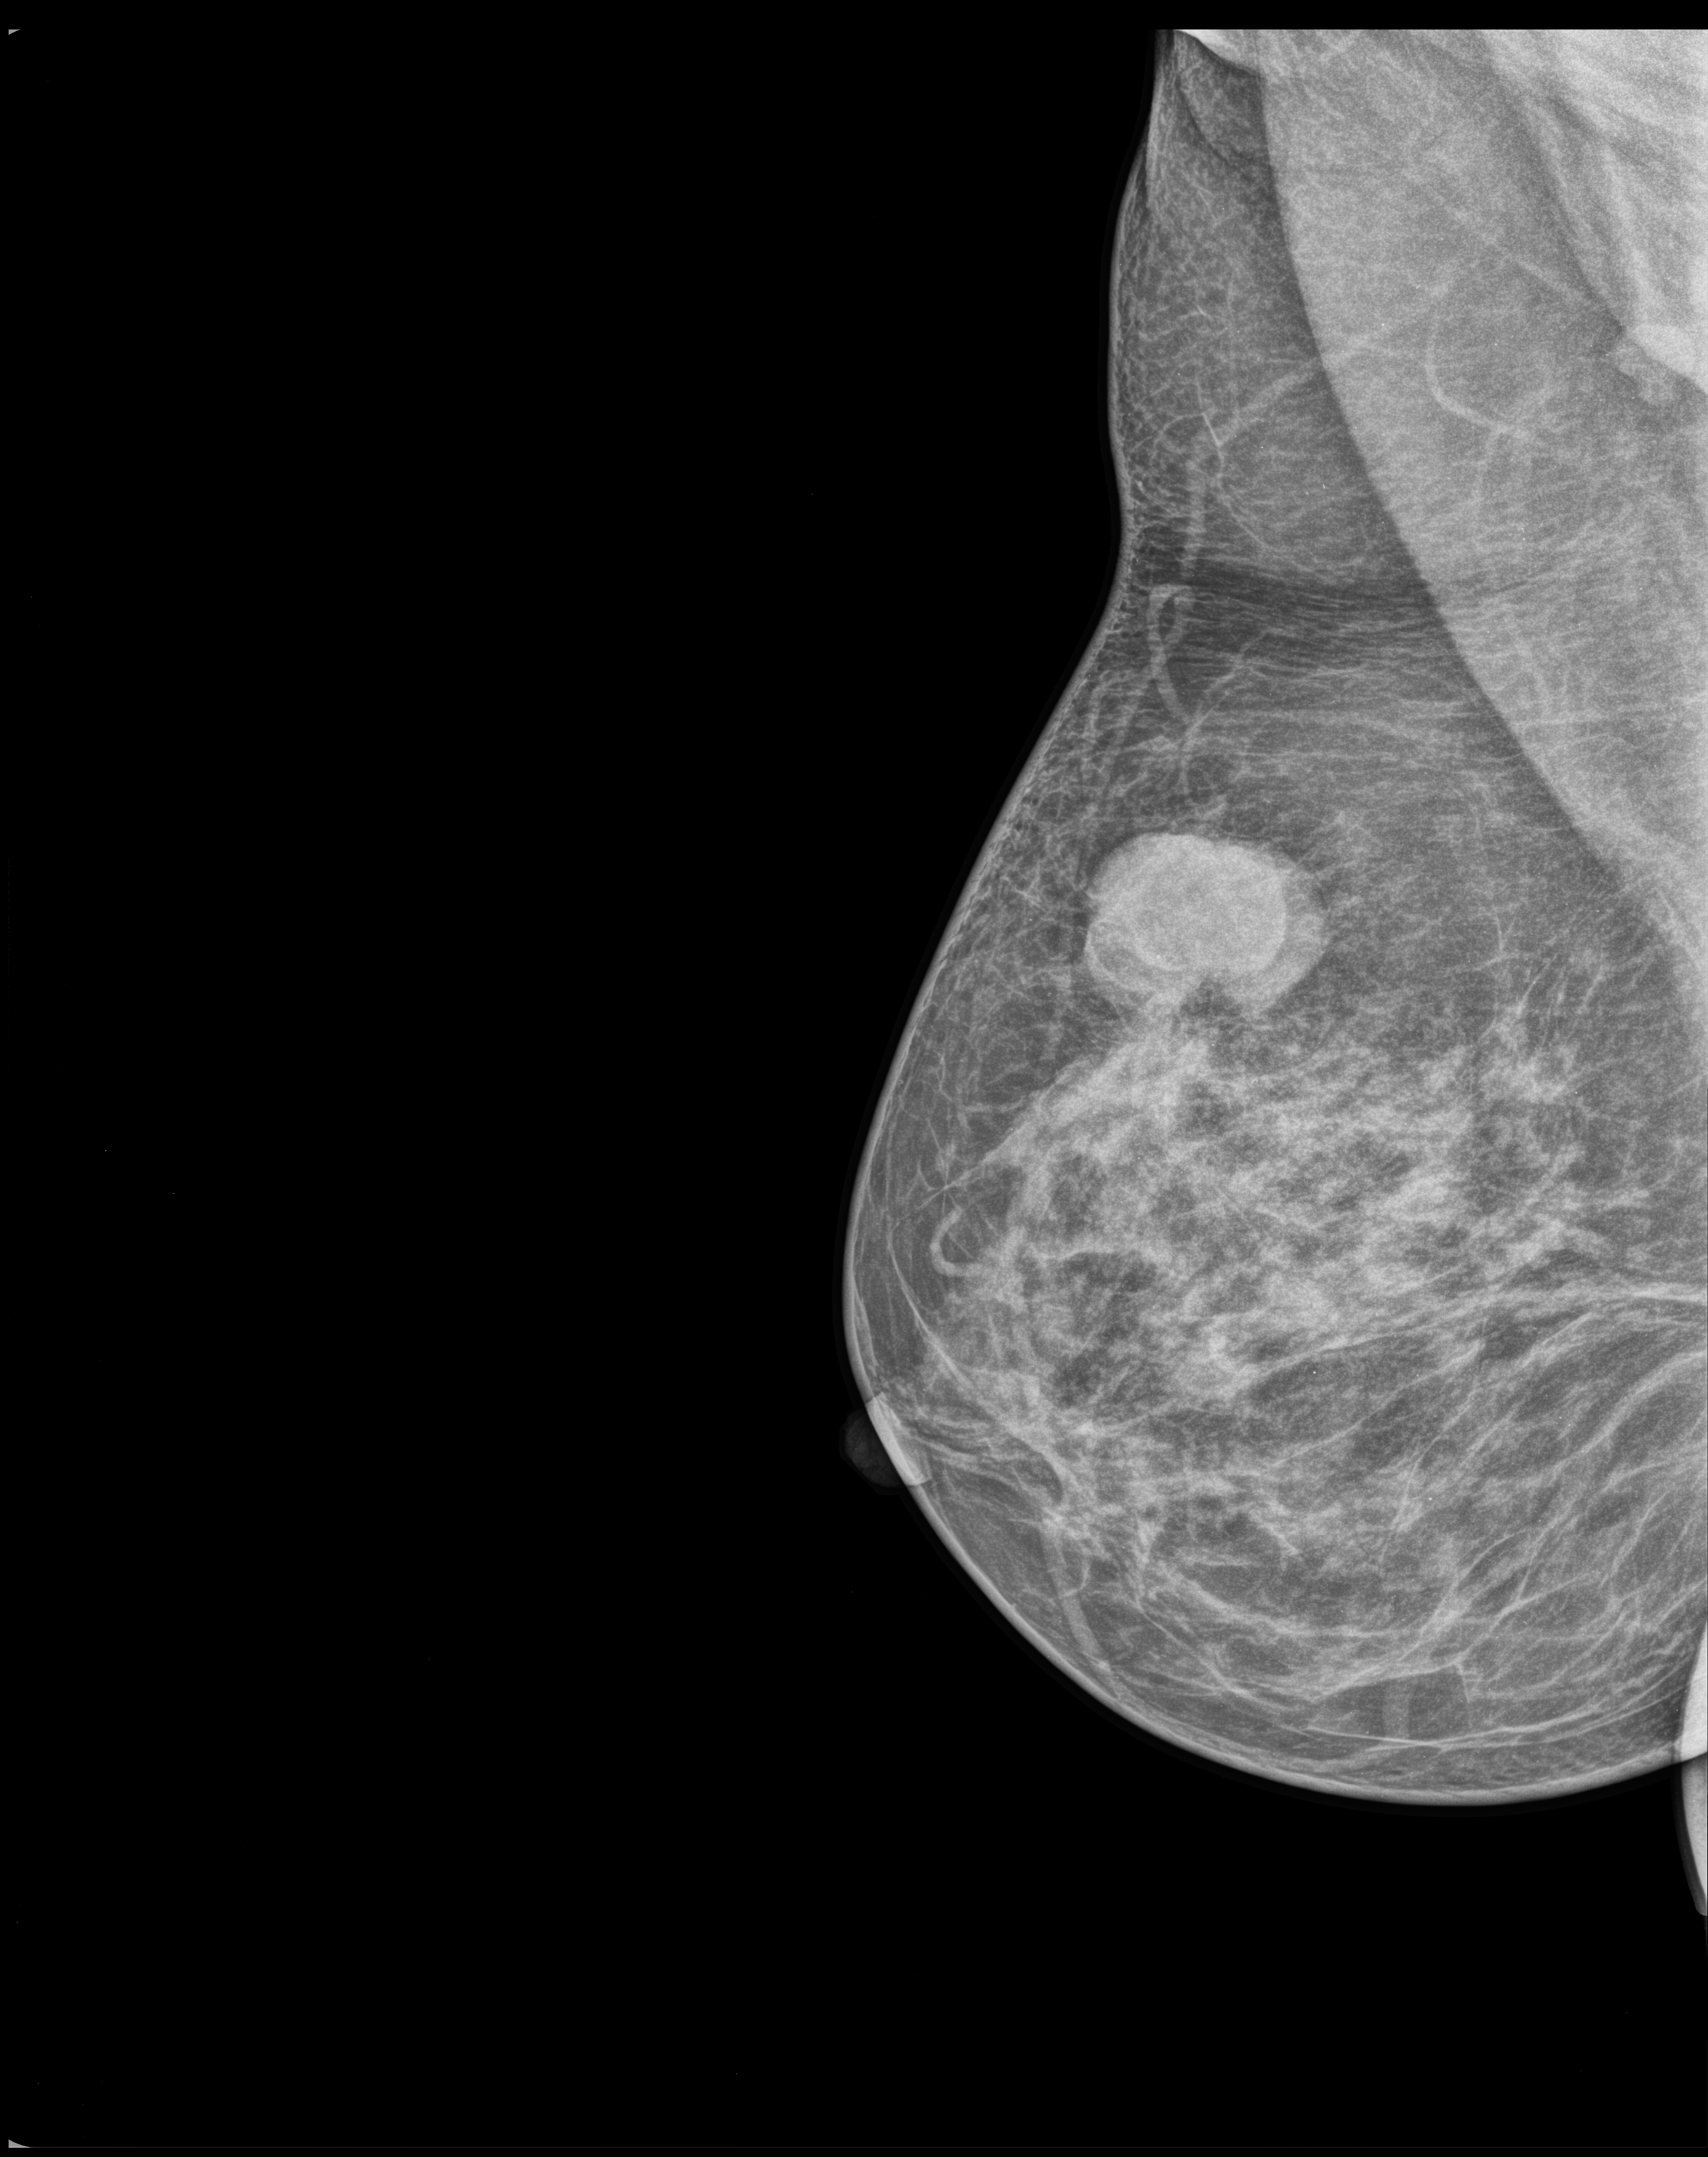
\includegraphics[width=0.48\linewidth]{../Reports/figures/normal/IMG086.png}\hfill
    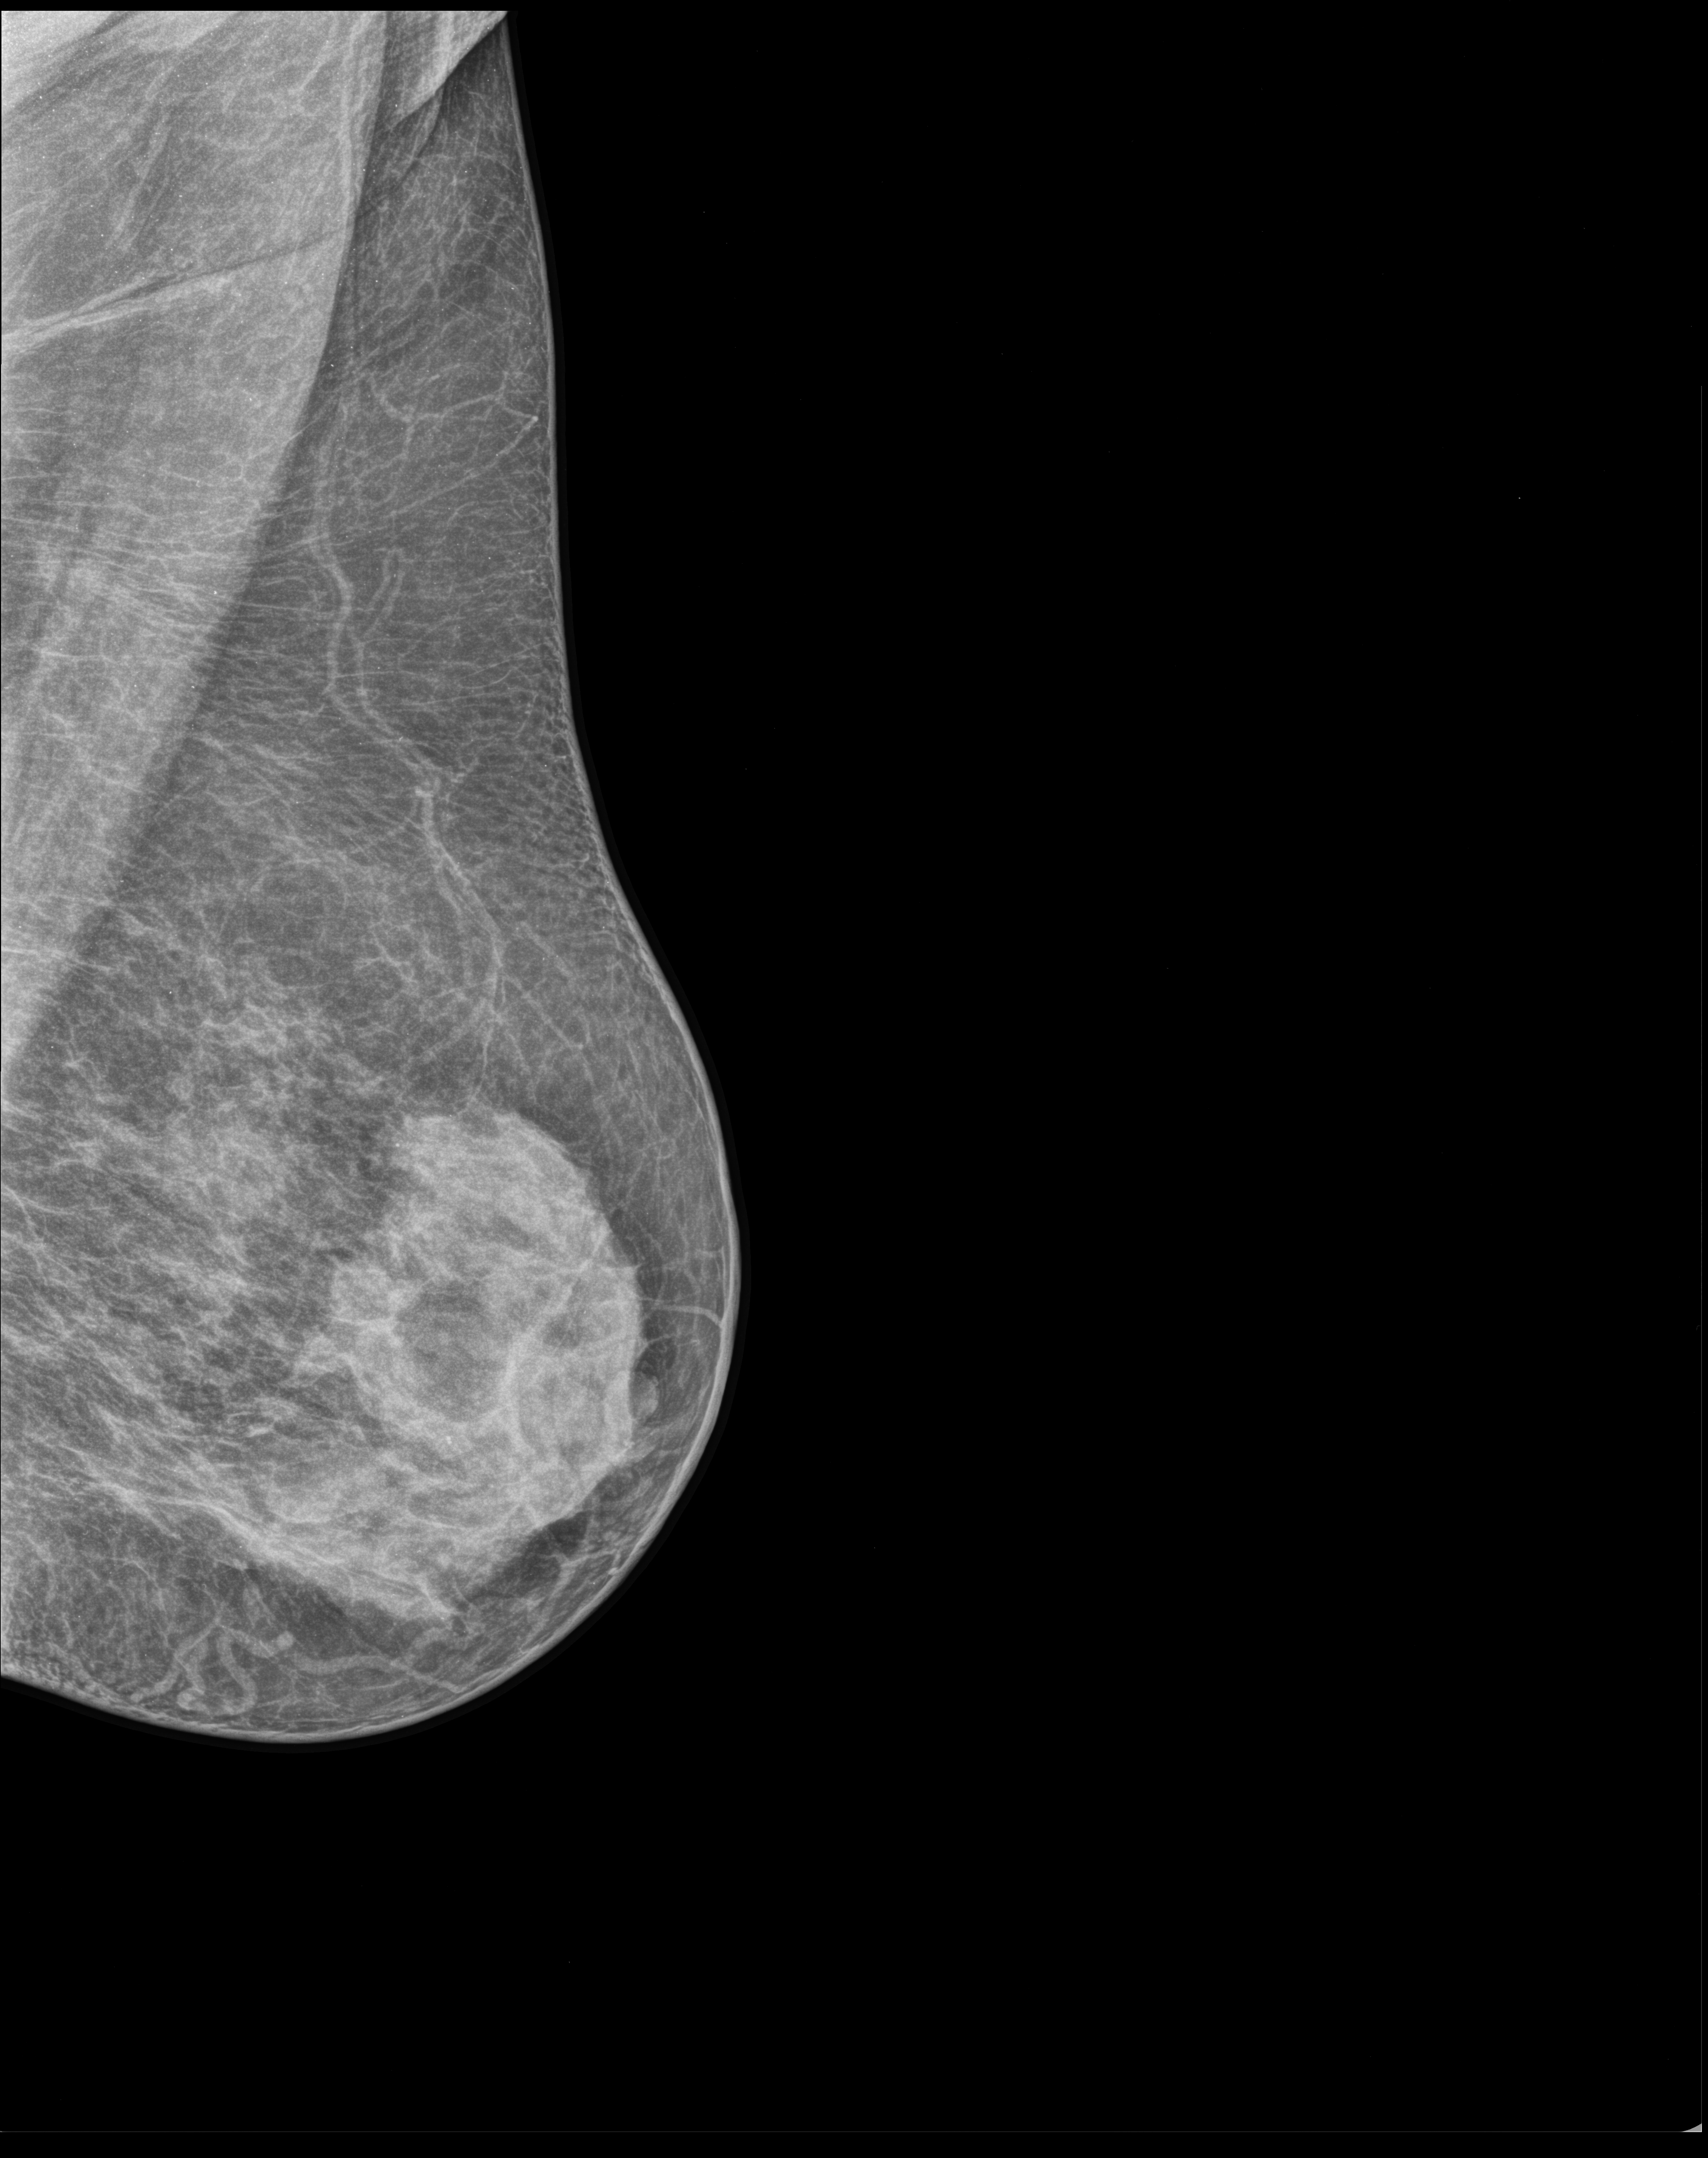
\includegraphics[width=0.48\linewidth]{../Reports/figures/normal/IMG187.png}\par\smallskip
    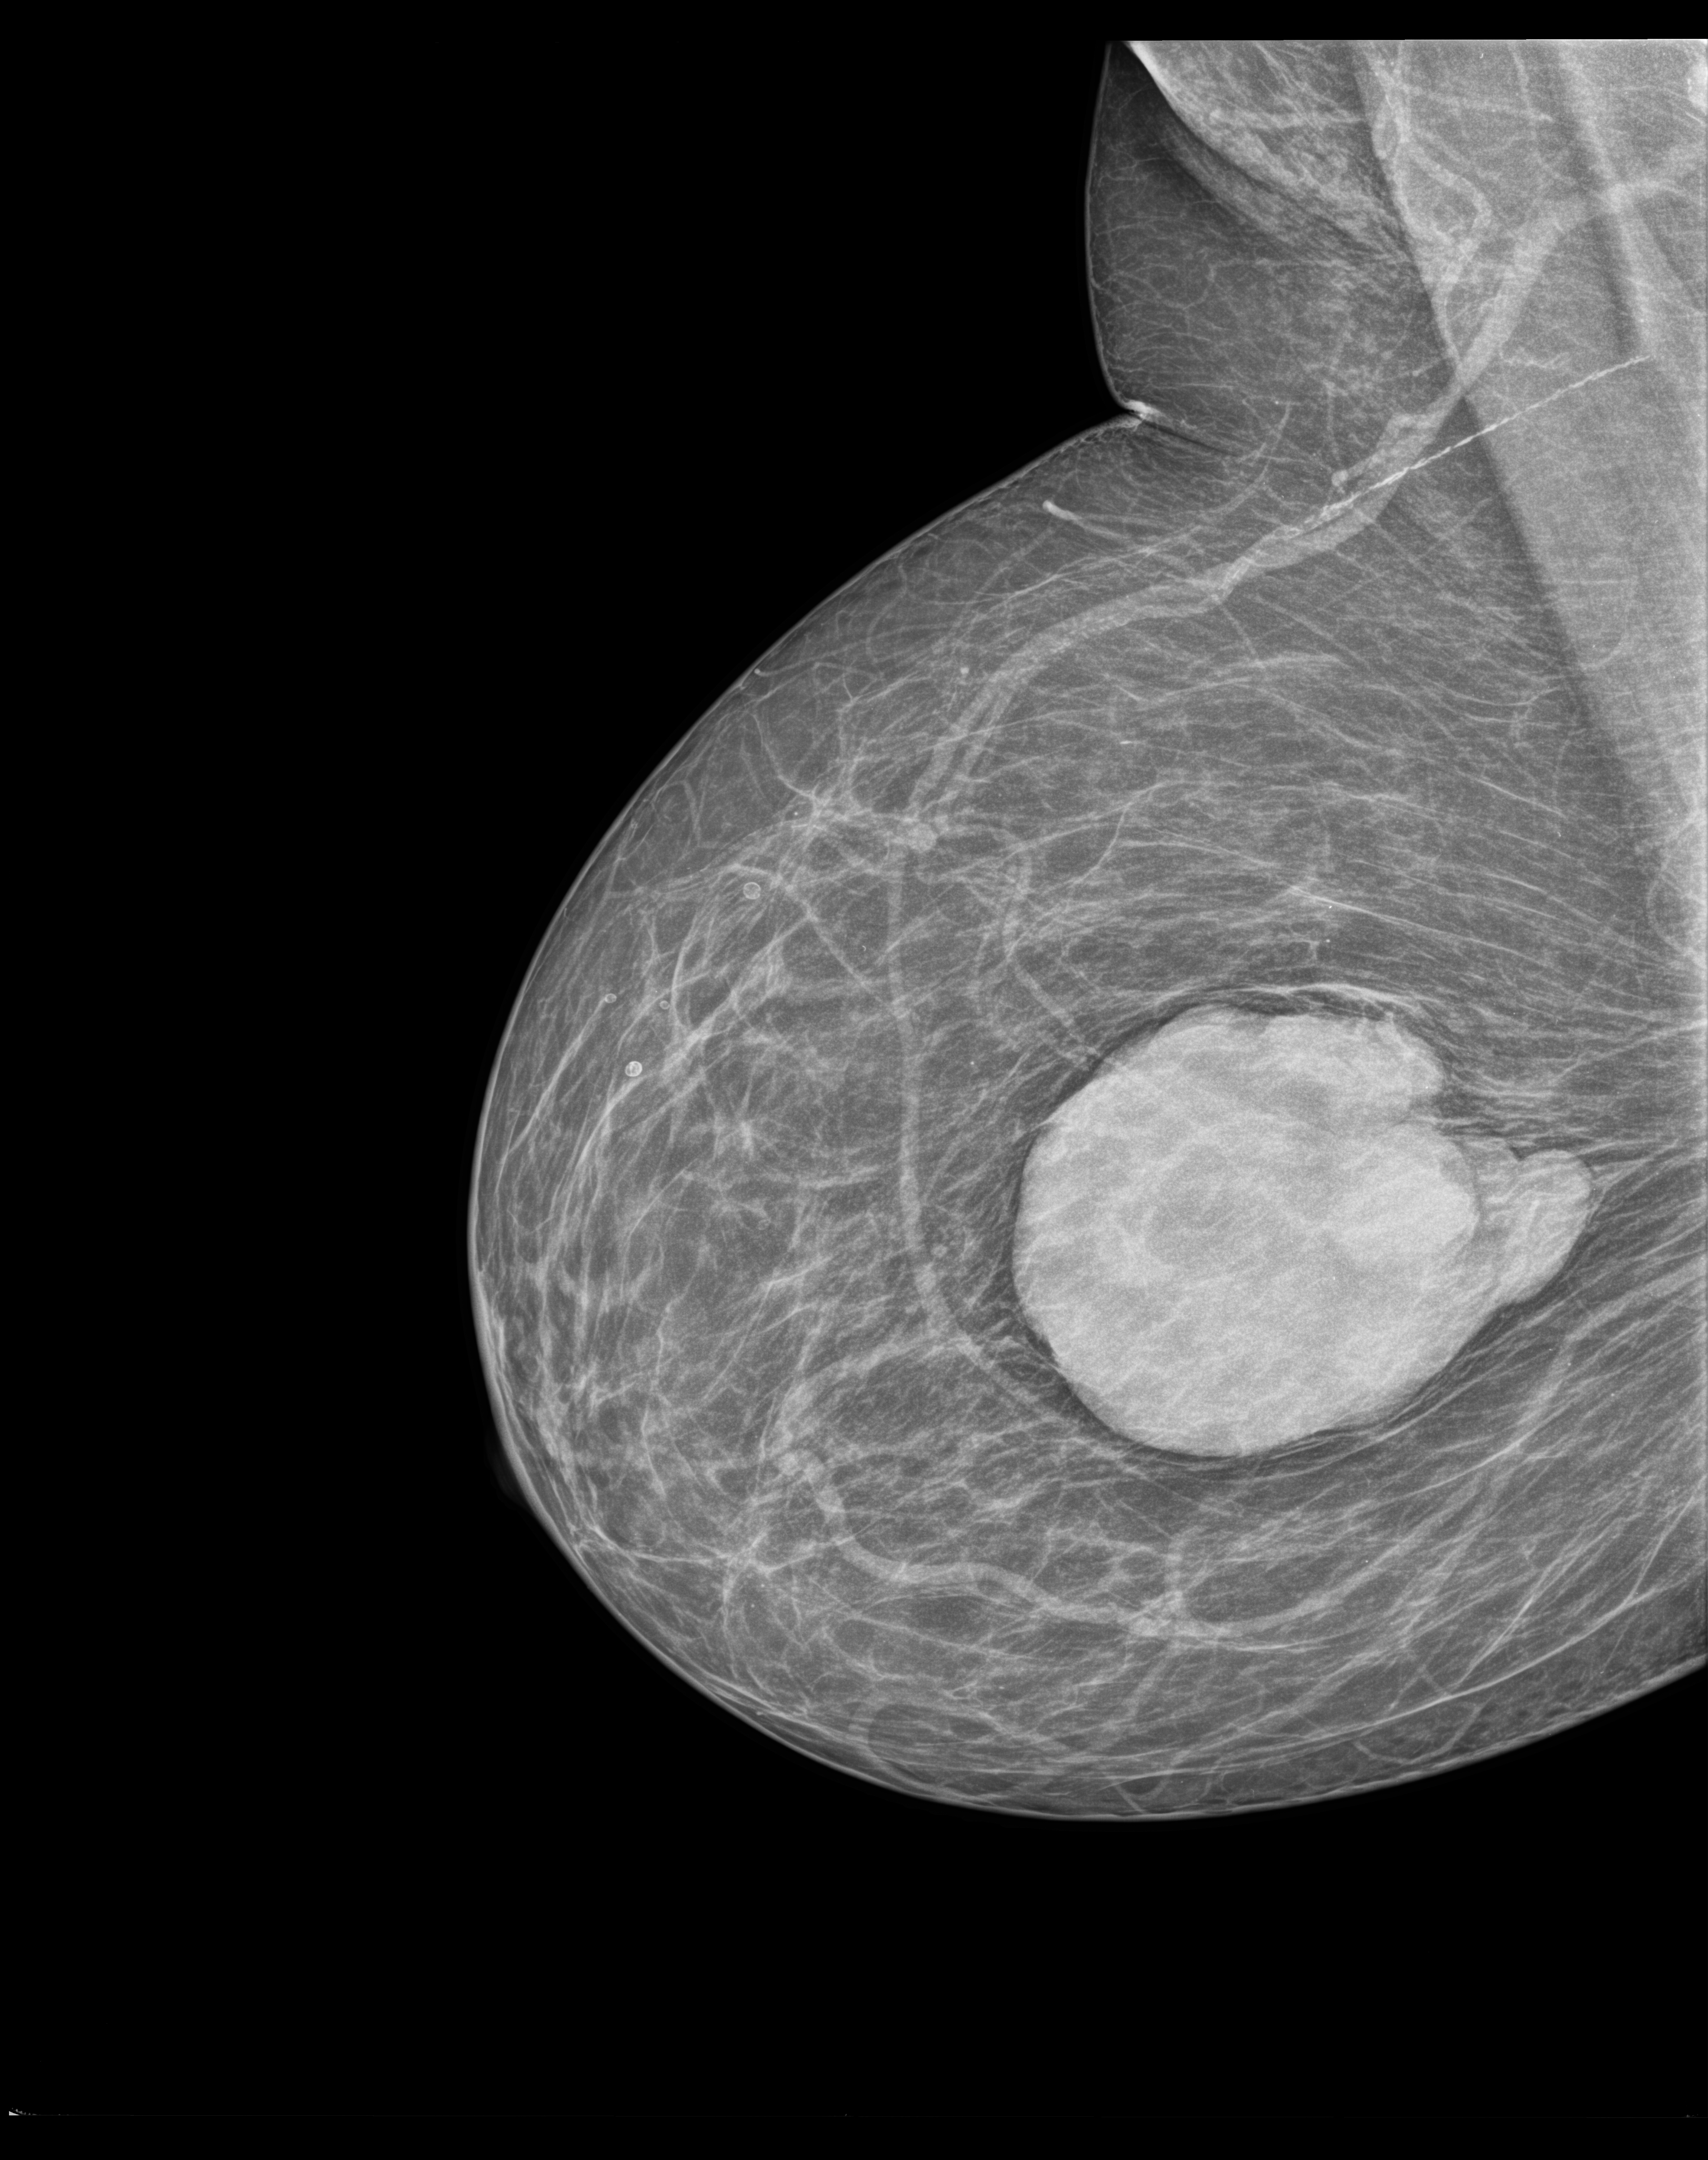
\includegraphics[width=0.48\linewidth]{../Reports/figures/normal/IMG440.png}\hfill
    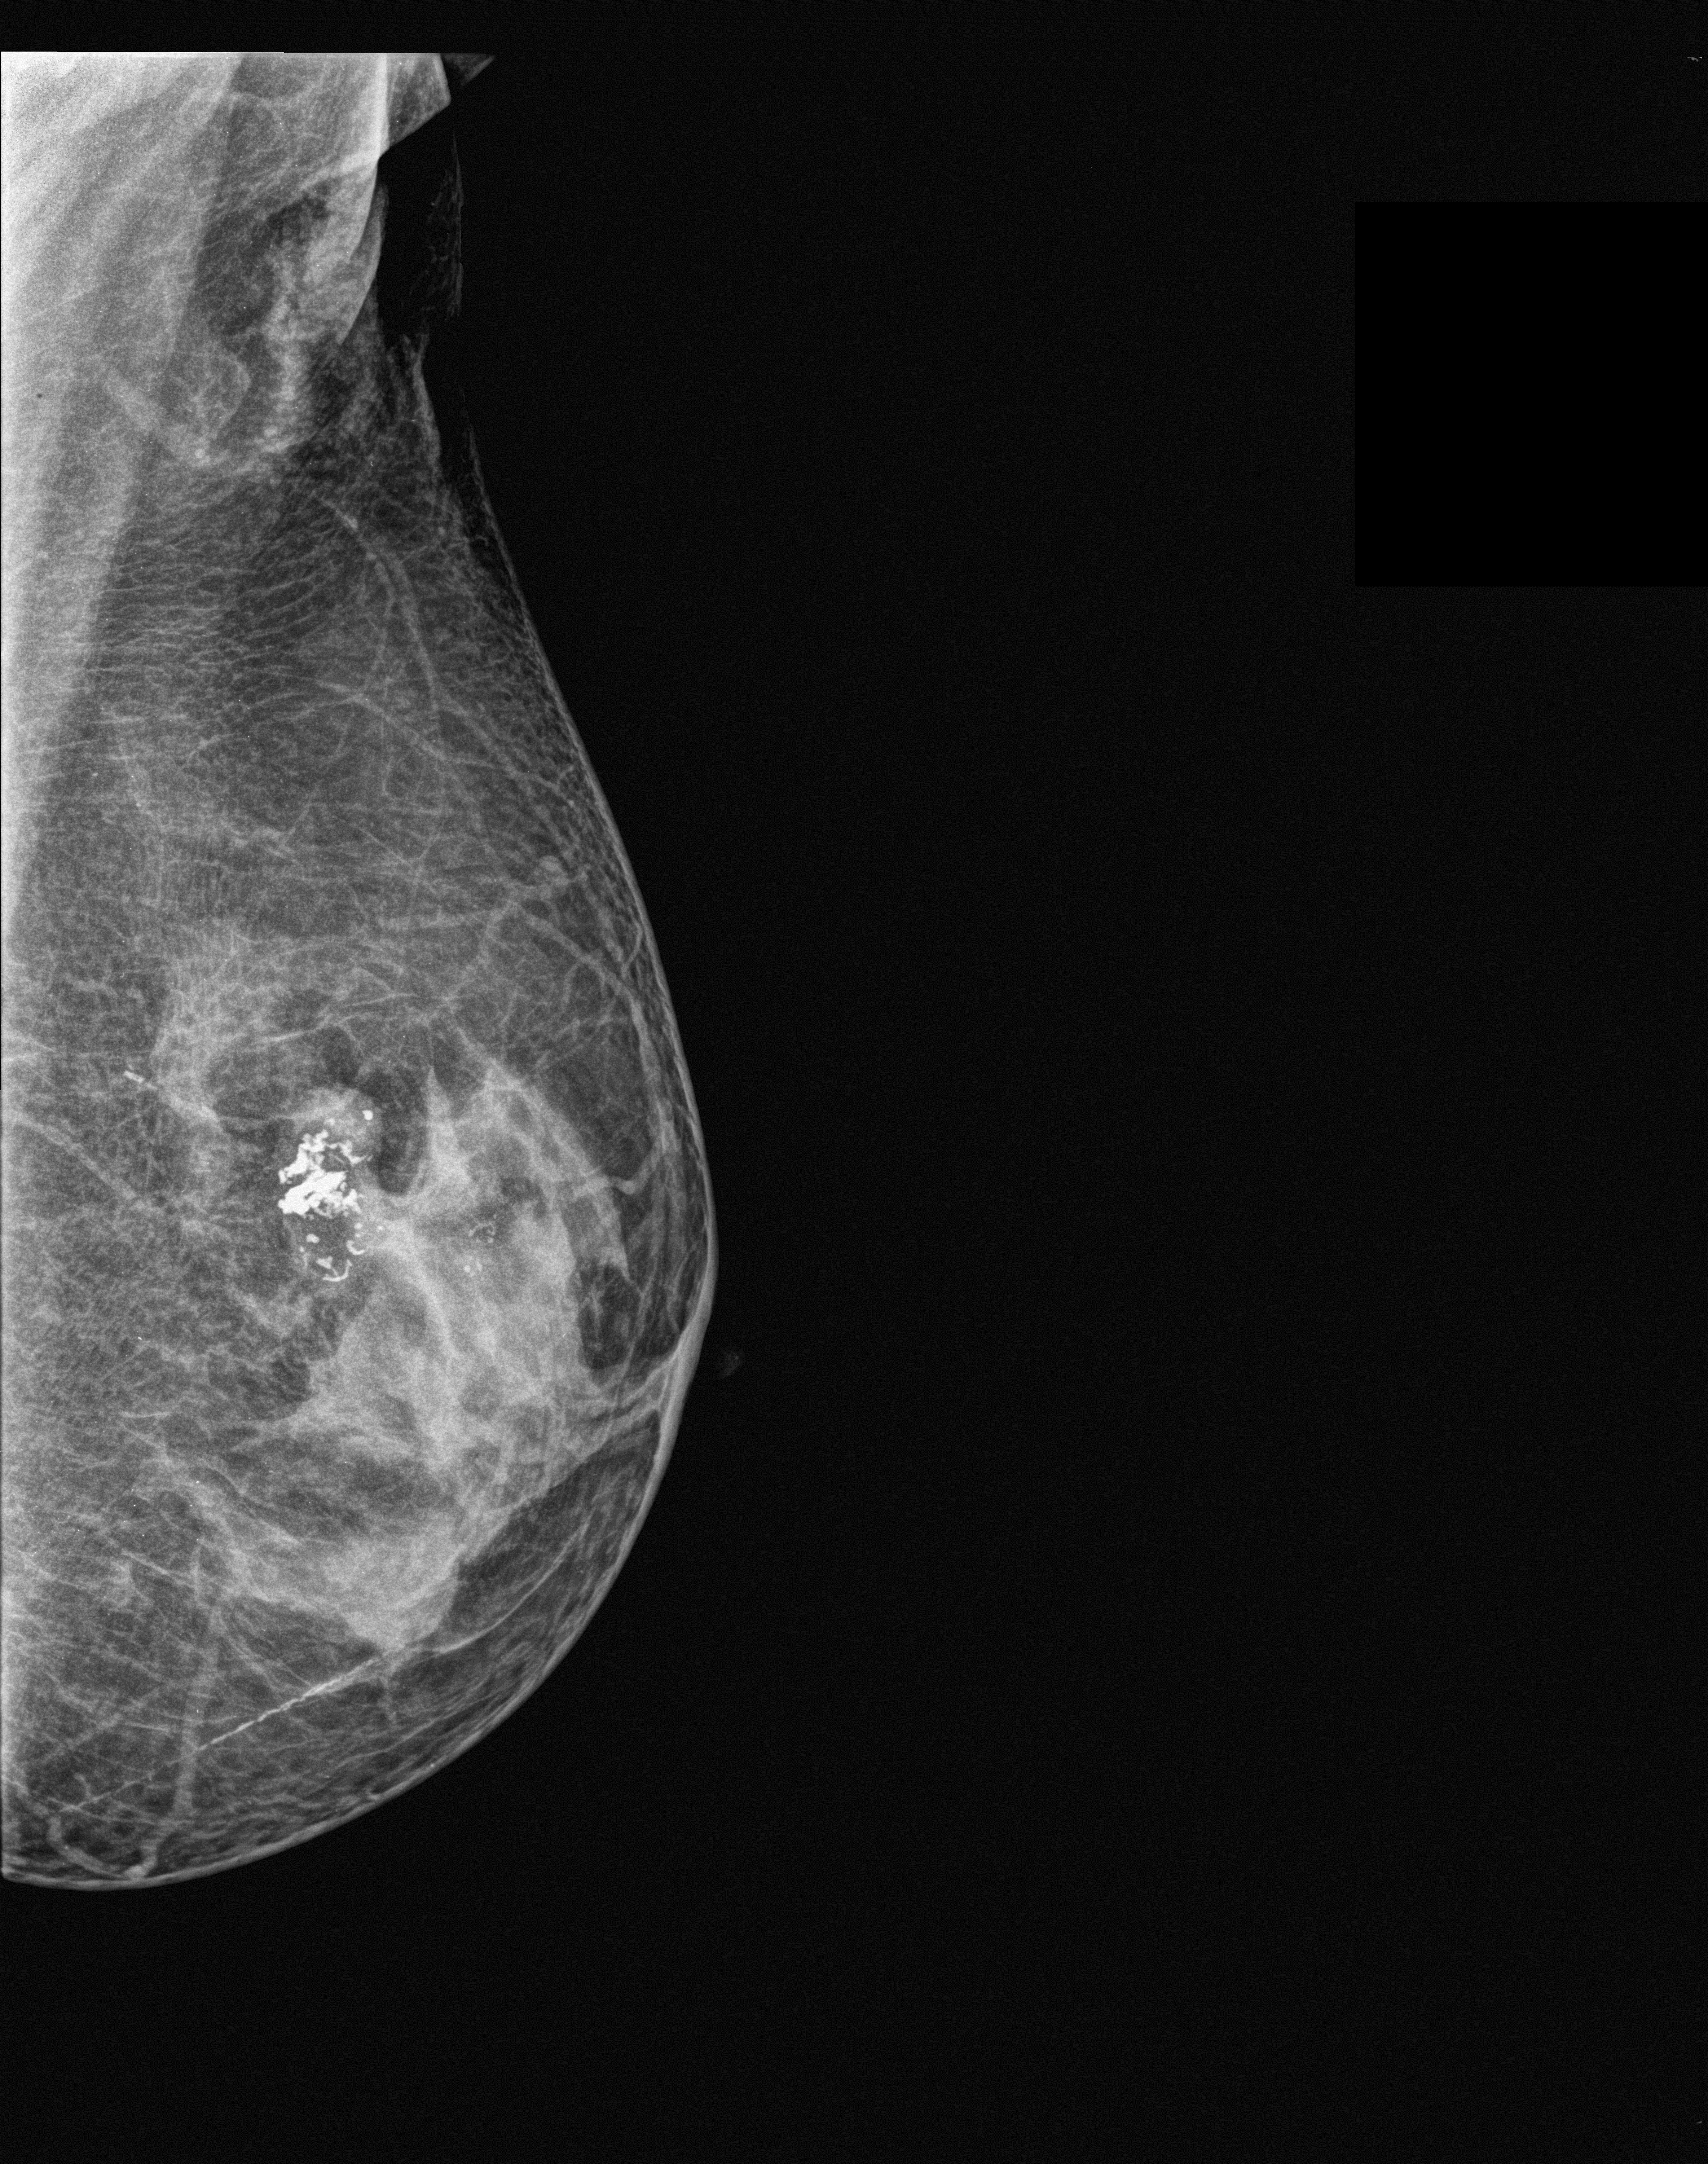
\includegraphics[width=0.48\linewidth]{../Reports/figures/normal/IMG459.png}
    \caption{Examples of normal-labeled images that still contain visually suspicious structure. These cases motivate the use of interpretable kernels and heatmap-based inspection during model development.}
    \label{fig:normalchallenging}
\end{figure}

\section{Patch Extraction and Splitting}
The pipeline extracts fixed-size patches from annotated regions and from background regions outside lesions. The extraction stage is configured through structured configuration objects. The default extraction uses patient-level splitting, a patch size of 128, positive-coverage thresholds for lesion-centered patches, and negative-coverage thresholds for background patches. These design choices aim to reduce leakage between train and evaluation subsets while keeping the patch labels structurally meaningful.

The current split used by the structured pipeline contains the counts shown in Table~\ref{tab:patchcounts}. The imbalance between inside and outside counts is modest and reflects the pragmatic trade-off between lesion sampling and background availability.

\begin{table}[H]
\centering
\caption{Patch counts in the train/validation/test split used by the repository pipeline.}
\label{tab:patchcounts}
\begin{tabular}{lcc}
\toprule
Split & Inside patches & Outside patches \\
\midrule
Train & 2900 & 3430 \\
Validation & 1080 & 790 \\
Test & 1040 & 830 \\
\bottomrule
\end{tabular}
\end{table}

\section{Pipeline Evolution During the Project}
The final structured pipeline emerged through iterative corrections to data preparation and visualization. Patch extraction was tightened to reduce leakage and label noise: positives were tied more strictly to lesion masks, negatives were split into near and far background groups with coverage limits, patient-level train/validation/test splitting was introduced, and dark or low-information patches were filtered out. These changes are methodologically significant because a large part of low-data performance comes from preventing mislabeled or redundant samples from dominating the representation.

The project also corrected an important class-definition issue. Instead of using only healthy-looking regions from malignant images as negatives, the later pipeline includes genuinely healthy slides as well. This matters because background tissue from malignant images can still carry subtle acquisition or context cues. Using healthy slides broadens the notion of ``outside'' tissue and yields a cleaner negative class.

A later refinement corrected the heatmap visualizer, which made the localization behavior much more trustworthy. This was an important turning point: once the visual outputs became reliable, small explicit-kernel models could be judged not only by patch classification but also by whether they localized clinically plausible regions.

These early adjustments explain an otherwise puzzling pattern in the repository: later numerical gains do not come only from changing the kernels themselves. They also depend on cleaning the data pipeline, correcting visualization, and making the positive/negative sampling policy more defensible.

\section{Baseline Kernel-bank Pipeline}
The baseline method converts image patches into scalar response features using a bank of handcrafted convolutional kernels. The structured implementation exposes this design explicitly in the configuration:
\begin{itemize}
    \item nine kernel families: Gaussian, anisotropic Gaussian, difference of Gaussians, Laplacian of Gaussian, Gabor, HOG-like, GLCM-inspired, LBP-inspired, and MRF-inspired kernels;
    \item configurable bank size per family;
    \item configurable response functions, selection strategies, and classifiers.
\end{itemize}

The overall pipeline can be summarized as follows:
\begin{enumerate}[label=\arabic*.]
    \item Extract lesion and non-lesion patches from the image corpus.
    \item Generate a large parameterized bank of 2D kernels.
    \item Convolve each patch with every kernel and summarize each response map into a scalar feature.
    \item Rank kernels by discriminative power and select a subset adaptively.
    \item Train a lightweight classifier on the selected response features.
\end{enumerate}

This design keeps the representation transparent. Each feature corresponds to an actual visual filter, and the selected subset can be inspected directly.

\section{Response Computation}
For a patch $x$ and kernel $K_j$, the baseline response stage computes a convolution map and reduces it to a scalar score. Early experiments use response functions such as absolute maximum or mean absolute response. Let $R_j(x)$ denote the scalar response of kernel $j$ on patch $x$. Then the feature vector for a patch is simply
\[
\phi(x) = [R_1(x), R_2(x), \ldots, R_m(x)].
\]

This scalar summarization is important both computationally and conceptually. It greatly reduces dimensionality, but it also discards some geometric detail. This later helps explain why visually different kernels can still yield similar classification behavior: if they induce similar patch rankings after scalar aggregation, a classifier may treat them as nearly interchangeable.

\section{Adaptive Selection and Classification}
Two main selection mechanisms are used in the project: MMR and ABESS. In the MMR variant, kernel relevance is balanced against redundancy. If $S$ is the set of already selected kernels and $j$ is a candidate, the selection score has the familiar form
\[
\text{MMR}(j) = \lambda \, \text{Rel}(j) - (1-\lambda)\max_{i \in S}\text{Sim}(i,j),
\]
where $\text{Rel}(j)$ measures discriminative utility and $\text{Sim}(i,j)$ measures similarity to already selected kernels \citep{goldstein1998mmr}. In the thesis setting, relevance is derived from response-based discrimination and similarity reflects redundancy within the candidate bank.

The selected responses are then passed to either logistic regression or a small multilayer perceptron, depending on the configuration. Most comparisons use logistic regression because it keeps the classifier stage simple and makes the effect of kernel design easier to interpret.

\section{Evaluation Criteria}
The main quantitative metrics reported throughout the repository are the area under the ROC curve (AUC) and accuracy at threshold 0.5. In addition, several experiments visualize confusion matrices, ROC/PR curves, selected kernels, and full-image heatmaps produced by sliding-window inference. These qualitative outputs are not cosmetic. They are part of the interpretability argument: they reveal whether stronger priors improve not only patch classification but also spatial localization behavior on full mammograms.

\chapter{Adaptive Kernel Design Framework}
\section{Overview}
The central methodological idea of the thesis is that kernel design itself can be adapted in several complementary ways. Instead of fixing one representation and only tuning the classifier, the project modifies where candidate kernels come from, which ones are kept, how they are combined, whether they respect rotational structure, and how compactly they can be parameterized.

\section{Adaptive Kernel-bank Selection}
The first level of adaptation operates on a large predefined bank. Rather than trusting any single handcrafted family, the pipeline mixes multiple families and lets data decide which kernels are most informative. This strategy is appropriate for low-volume data because it externalizes much of the modeling prior into the filter bank rather than attempting to learn every degree of freedom from scratch.

The adaptive step has two parts. The first is discriminative ranking, which quickly rejects clearly weak filters. The second is diversity-aware selection, which discourages the chosen set from collapsing onto near-duplicates. In practice, the compared runs show that MMR and ABESS lead to similar best-case AUC values, but MMR produces slightly stronger peak results in the settings emphasized here. The selection stage therefore acts as a regularizer on representation complexity: it keeps only those kernels that are simultaneously useful and not redundant.

\section{Adaptive Kernel Composition}
The second form of adaptation composes multiple selected kernels into a smaller number of aggregate filters. If the selected kernels are $\{K_i\}_{i=1}^n$ and the composition weights are $w_i$, a composite kernel has the form
\[
K_{\text{comp}} = \sum_{i=1}^{n} w_i K_i.
\]

This reduces the number of explicit features and can yield visually meaningful aggregate filters. However, the thesis results show that compression before classification introduces a trade-off. When per-kernel responses are first collapsed through a nonlinear statistic such as absolute maximum, the operation ``compose then respond'' is not equivalent to ``respond then classify''. As a result, some discriminative information is lost. The composition stage is therefore useful as an efficiency and interpretability mechanism, but it is not automatically performance-preserving.

\section{Adaptive Sampling of Kernel Parameters}
A third adaptive mechanism concerns how kernel parameters are sampled. Random sampling is the legacy baseline, but the structured code also supports Sobol quasi-Monte Carlo sampling and Latin hypercube sampling. The thesis focuses on Sobol sampling because low-discrepancy sequences cover bounded parameter spaces more uniformly than naive random draws \citep{sobol1967cube}. In a finite kernel-bank regime, this matters: better coverage of parameter space can improve the odds of discovering discriminative filters without increasing bank size excessively.

In conceptual terms, this is a form of adaptation at the search level rather than the model level. Under low-volume conditions, one cannot assume that broad random exploration will always be efficient. QMC sampling imposes more structure on the search itself.

\section{Adaptive Rotational Design}
Mammographic lesions often display structure that is not fully orientation-specific, which motivates the study of rotational behavior. The project investigates this question in two ways. First, it measures how much existing kernels and composite models change under rotation. Second, it constructs explicitly rotation-averaged kernels. If $K$ is a 2D kernel and $\operatorname{rot90}(K, r)$ denotes rotation by $90r$ degrees, the right-angle invariant version is
\[
K_{\text{RI}} = \frac{1}{4}\sum_{r=0}^{3}\operatorname{rot90}(K,r).
\]

This is a strict and transparent form of prior encoding. It removes orientation preference by construction rather than by data augmentation alone. The price is that orientation-specific information may also be removed. The experiments show both sides of this trade-off clearly.

\section{Adaptive Learned Radial Kernels}
The final and most important adaptation compresses the kernel itself into a radial parameterization. Instead of learning or selecting many free 2D filters, the model defines a kernel by ring-shaped basis functions $B_r$ and shell coefficients $f_r$:
\[
K(x,y) = \sum_{r=0}^{R} f_r B_r(x,y).
\]

This produces a one-dimensional profile over radius. Several versions of the radial model were investigated during development:
\begin{itemize}
    \item a seed-based radial optimization initialized from an existing learned kernel;
    \item a signed compact version with stronger support control;
    \item an independent signed radial model learned from scratch;
    \item a free signed ablation in which positivity and monotonicity were removed;
    \item a final signed radial model with a learnable effective radius.
\end{itemize}

The later signed versions change both the representation and the scoring function. Instead of using an absolute peak that may hide sign structure, they average the strongest signed responses:
\[
s(x;K) = \frac{1}{k}\sum_{p \in \operatorname{TopK}(|K * x|)} (K * x)_p.
\]
This encourages the score to depend on a consistent pattern rather than a single extreme activation.

\begin{verbatim}
# Signed top-k response (conceptual)
R = conv2d(patch, kernel)
idx = topk_indices(abs(R), k)
score = mean(R[idx])
\end{verbatim}

The final learnable-radius version also introduces a differentiable support parameter. The shell coefficients remain L2-normalized, but they are allowed to take both positive and negative values, and the optimizer can expand or contract the effective radial support jointly with the profile. The radial line of work is the thesis endpoint because it transforms the original broad kernel-bank idea into a compact, interpretable, explicitly regularized model with far fewer degrees of freedom.

\chapter{Results and Discussion}
\section{Reading the Results}
The results are best read as a chronological development path. The project begins with sparse bank selection, then tests stronger compression and search strategies, then studies rotational structure, and finally moves into progressively more structured radial models. Not every stage uses exactly the same split, pooling rule, or optimization objective, so the chapter distinguishes between two kinds of comparison:
\begin{itemize}
    \item \textbf{matched comparisons}, where runs were designed as direct alternatives under the same experimental setup;
    \item \textbf{developmental comparisons}, where runs illustrate how one modeling issue was identified and then addressed in the next step.
\end{itemize}

This distinction keeps the narrative honest. The goal is not to force all runs into one leaderboard, but to show which lessons remain stable while the representation becomes smaller, more constrained, and more interpretable.

\section{Baseline Selection Results}
The development begins with adaptive selection from a large handcrafted kernel bank. Table~\ref{tab:selectionresults} summarizes representative MMR and ABESS outcomes under the same general selection setup.

\begin{table}[H]
\centering
\caption{Representative matched results for adaptive kernel-bank selection.}
\label{tab:selectionresults}
\begin{tabular}{lcccc}
\toprule
Configuration & Selector & Selected kernels & Test AUC & Test ACC \\
\midrule
Sparse MMR subset & MMR & 3 & 0.9239 & 0.7914 \\
Expanded sparse MMR subset & MMR & 5 & 0.9234 & 0.7594 \\
Dense MMR subset & MMR & 200 & 0.9180 & 0.7909 \\
Very dense MMR subset & MMR & 300 & 0.8927 & 0.8182 \\
Dense ABESS subset & ABESS & 200 & 0.9236 & 0.7690 \\
Very dense ABESS subset & ABESS & 300 & 0.8966 & 0.8032 \\
\bottomrule
\end{tabular}
\end{table}

Two points are immediately visible. First, the best AUC does not come from the largest selected set. A small MMR subset of three kernels already reaches a test AUC of 0.9239. Second, increasing feature count shifts the operating point: the 300-kernel MMR model reduces AUC but increases thresholded accuracy relative to the smaller sparse models. This suggests that adaptive selection is not only a relevance filter but also a mechanism for controlling the complexity-versus-stability trade-off of the final classifier.

The corresponding kernel visualizations show that the selected sets are dominated by Gaussian, anisotropic Gaussian, and Gabor-like structures, which is consistent with the texture-and-shape emphasis of mammographic lesions. Figure~\ref{fig:selectedkernels} illustrates one representative selected-kernel panel.

\begin{figure}[H]
    \centering
    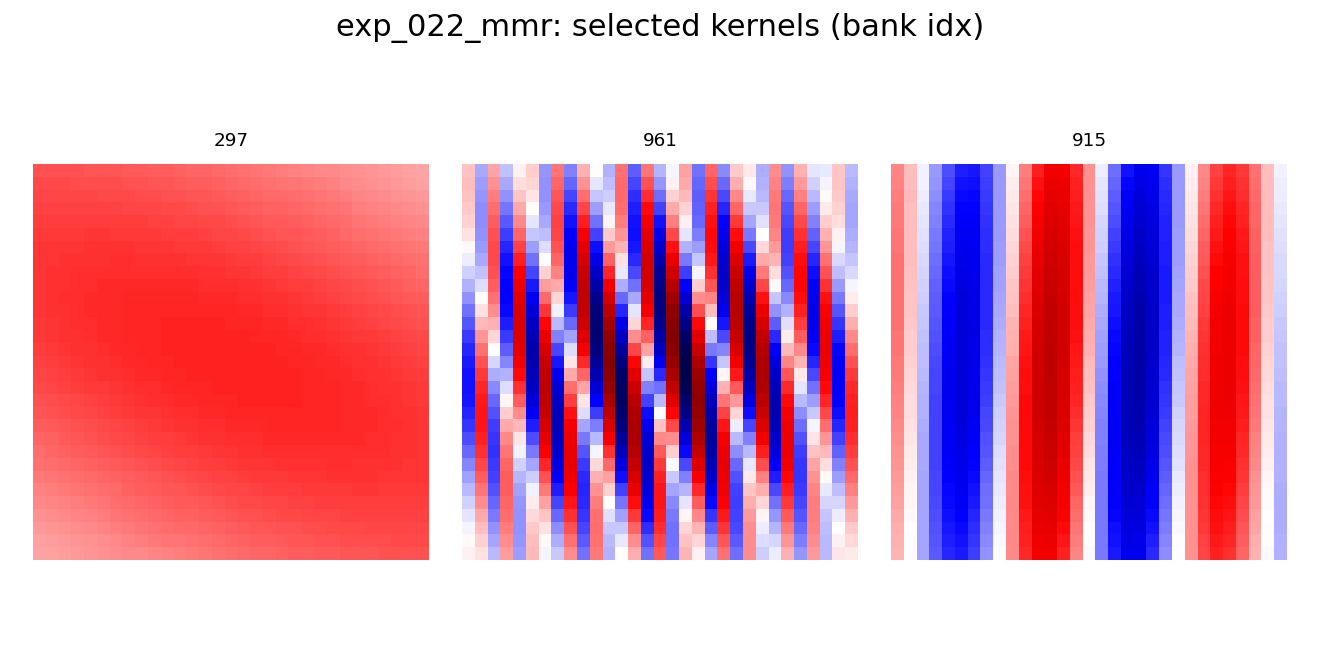
\includegraphics[width=0.92\linewidth]{../Reports/figures/exp_022_mmr_selected_kernels.png}
    \caption{Representative selected-kernel visualization for the sparse MMR baseline. The explicit filters are part of the interpretability advantage of the pipeline.}
    \label{fig:selectedkernels}
\end{figure}

\section{Early Heatmap Validation and Qualitative Error Analysis}
Before the later compression steps were attempted, an early sparse branch established an important qualitative checkpoint. After the patch extraction and heatmap rendering were corrected, a small 5-kernel model already produced meaningful lesion localization instead of only patch-level separation. This mattered because it showed that sparse explicit kernels could remain spatially informative.

Figure~\ref{fig:exp019heatmaps} reproduces representative full-image heatmaps from that stage. The malignant cases show concentrated activation around suspicious regions, while the normal cases remain more diffuse or suppressed. This kind of visual inspection directly influenced later decisions to keep lightweight classifiers and interpretable filter responses rather than optimizing only leaderboard numbers.

\begin{figure}[H]
    \centering
    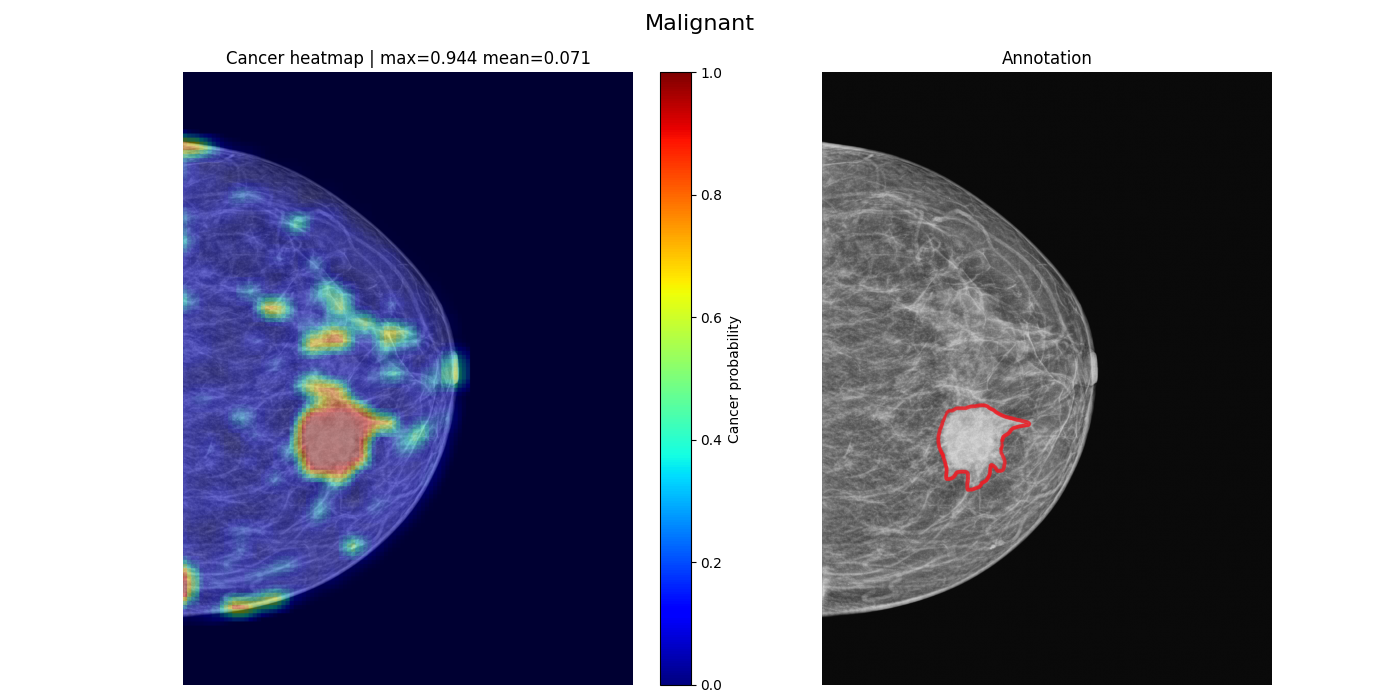
\includegraphics[width=0.48\linewidth]{../results/exp_019/heatmaps/IMG483.tif_heatmap.png}\hfill
    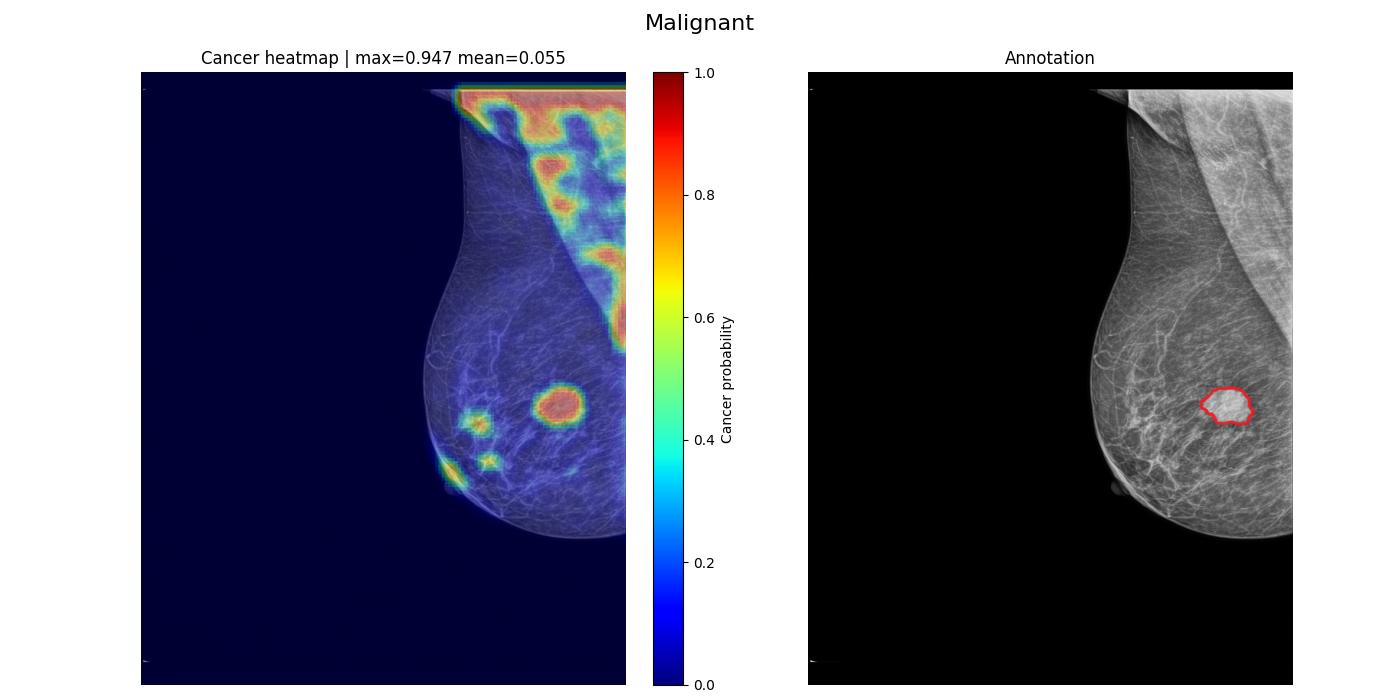
\includegraphics[width=0.48\linewidth]{../results/exp_019/heatmaps/IMG033.tif_heatmap.png}\par\smallskip
    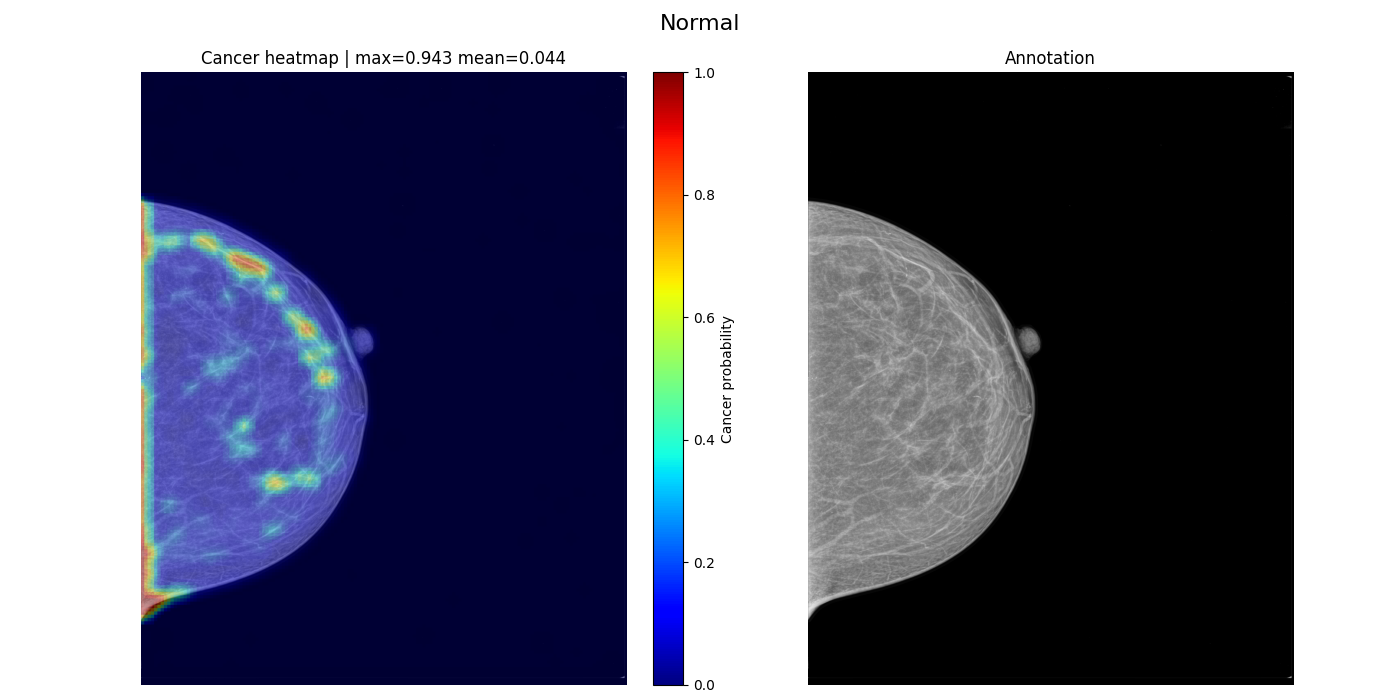
\includegraphics[width=0.48\linewidth]{../results/exp_019/heatmaps/IMG263.tif_heatmap.png}\hfill
    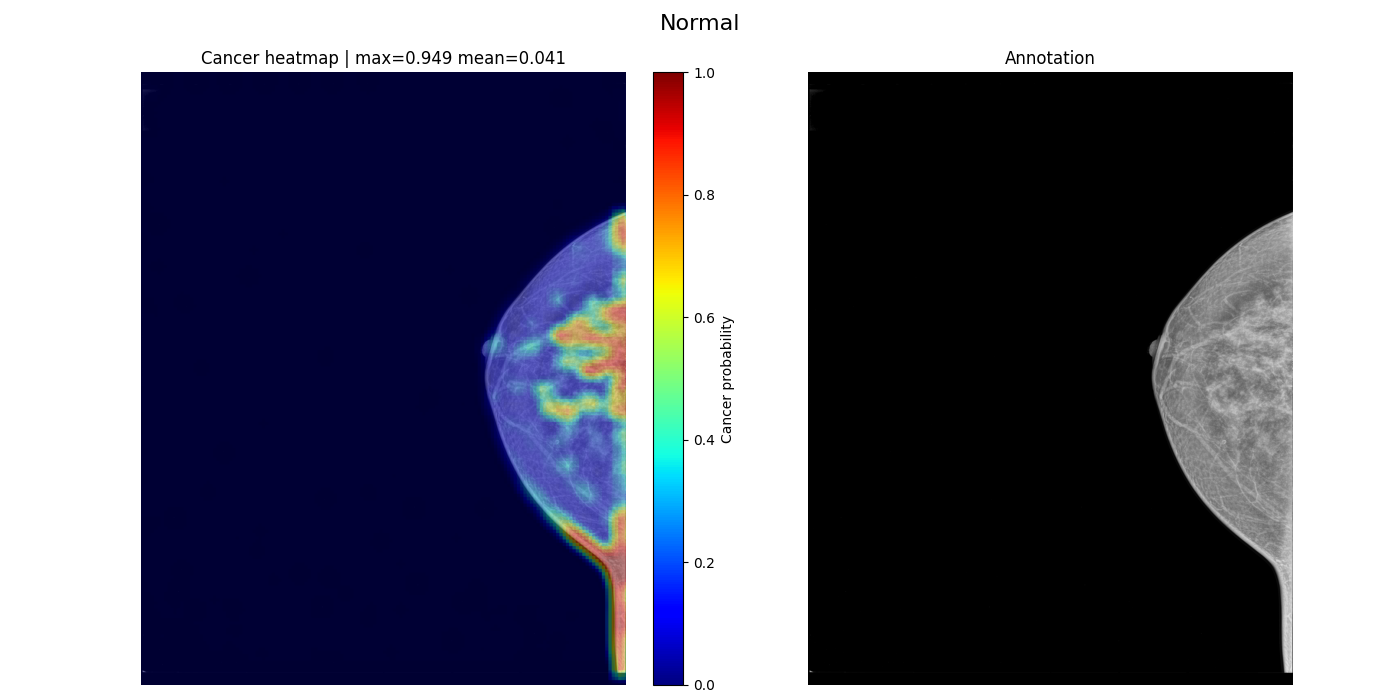
\includegraphics[width=0.48\linewidth]{../results/exp_019/heatmaps/IMG351.tif_heatmap.png}
    \caption{Representative malignant and normal heatmaps from the early sparse-kernel stage. These figures were important for validating that a very small set of explicit kernels could still localize meaningful tissue structure.}
    \label{fig:exp019heatmaps}
\end{figure}

This early phase also exposed an unavoidable difficulty of the case study: some normal-labeled images look visually suspicious. That ambiguity is exactly why the thesis emphasizes interpretable feature design and qualitative review together. A model can be penalized by the nominal label even when its heatmap appears visually reasonable, and such cases should be treated as a dataset limitation rather than as pure model failure.

\section{Reduced-bank Sparse Variants}
The next question was how aggressively the bank could be reduced before the classifier became too weak. Table~\ref{tab:reducedbank} summarizes representative reduced-bank MMR variants.

\begin{table}[H]
\centering
\caption{Reduced-bank MMR variants.}
\label{tab:reducedbank}
\small
\begin{tabular}{lcccc}
\toprule
Configuration & Kernels per family & Selected kernels & Test AUC & Test ACC \\
\midrule
One per family, 1 selected & 1 & 1 & 0.9157 & 0.8449 \\
Three per family, 1 selected & 3 & 1 & 0.9179 & 0.8428 \\
Three per family, 3 selected & 3 & 3 & 0.9101 & 0.8417 \\
Ten per family, 3 selected & 10 & 3 & 0.9032 & 0.8449 \\
\bottomrule
\end{tabular}
\normalsize
\end{table}

These runs are interesting because they retain strong thresholded accuracy despite drastically reducing the bank size. Relative to the strongest AUC-focused sparse baseline, they lose some ranking performance, but they show that the pipeline does not require hundreds of filters to remain useful. In a low-data setting, this is valuable evidence: compactness can be increased very aggressively before performance collapses.

\begin{figure}[H]
    \centering
    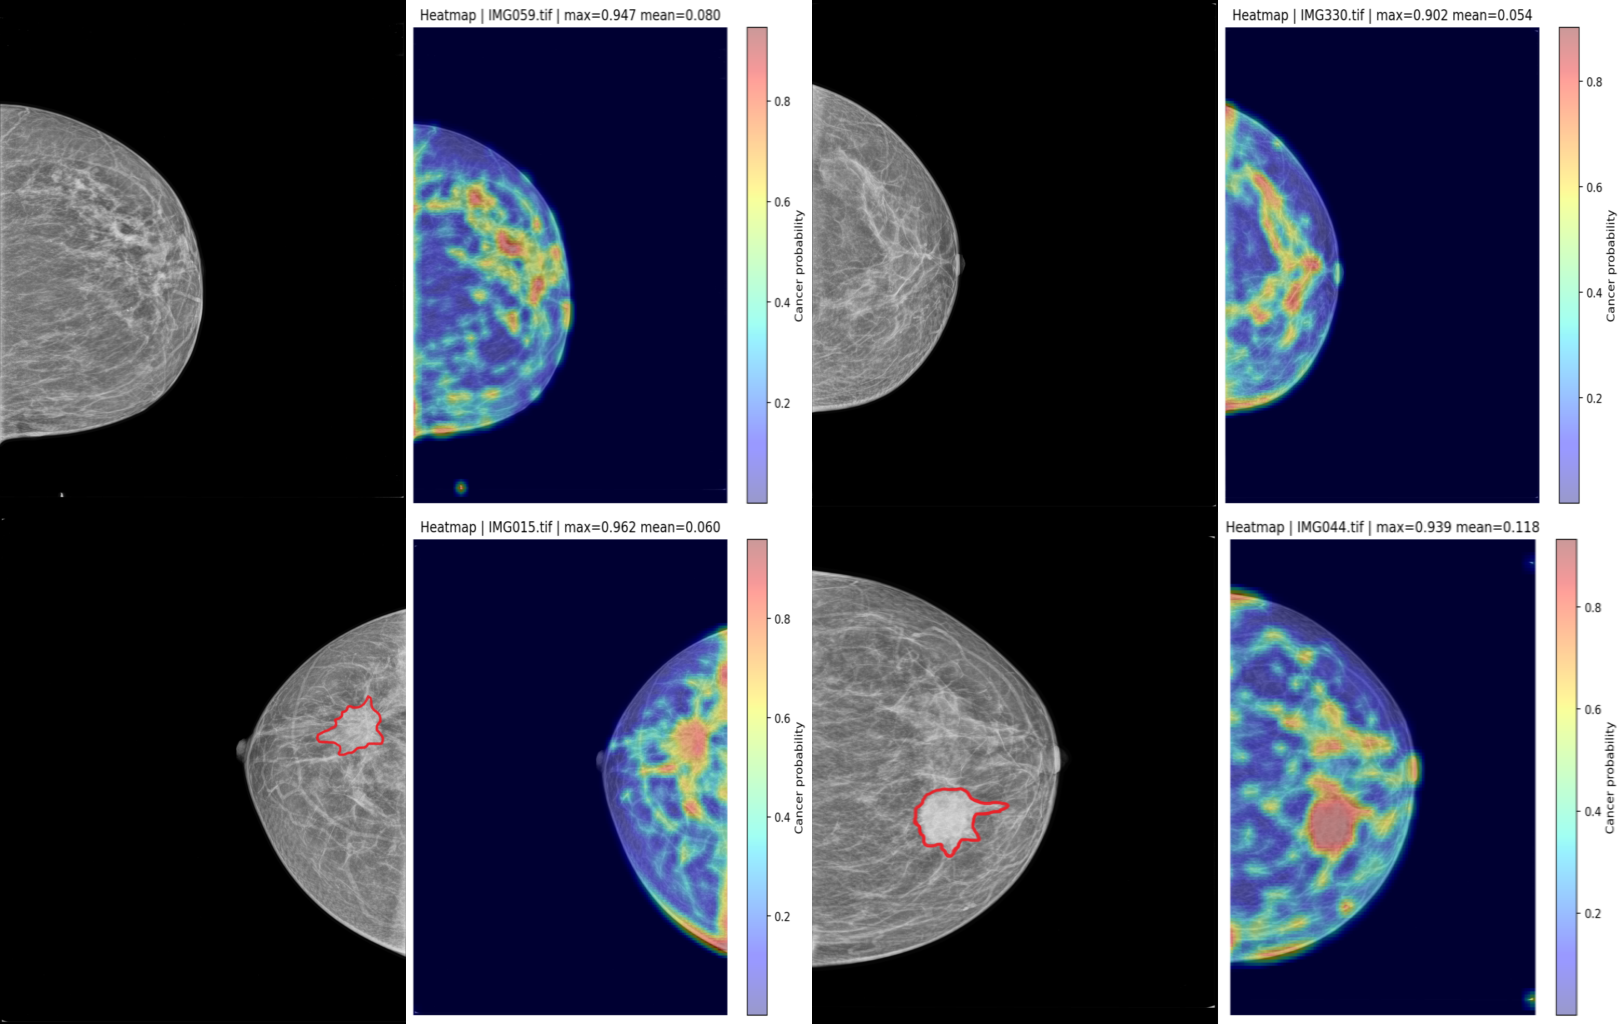
\includegraphics[width=0.48\linewidth]{../results/exp_022_mmr_n1_k1/heatmaps_side_by_side.png}\hfill
    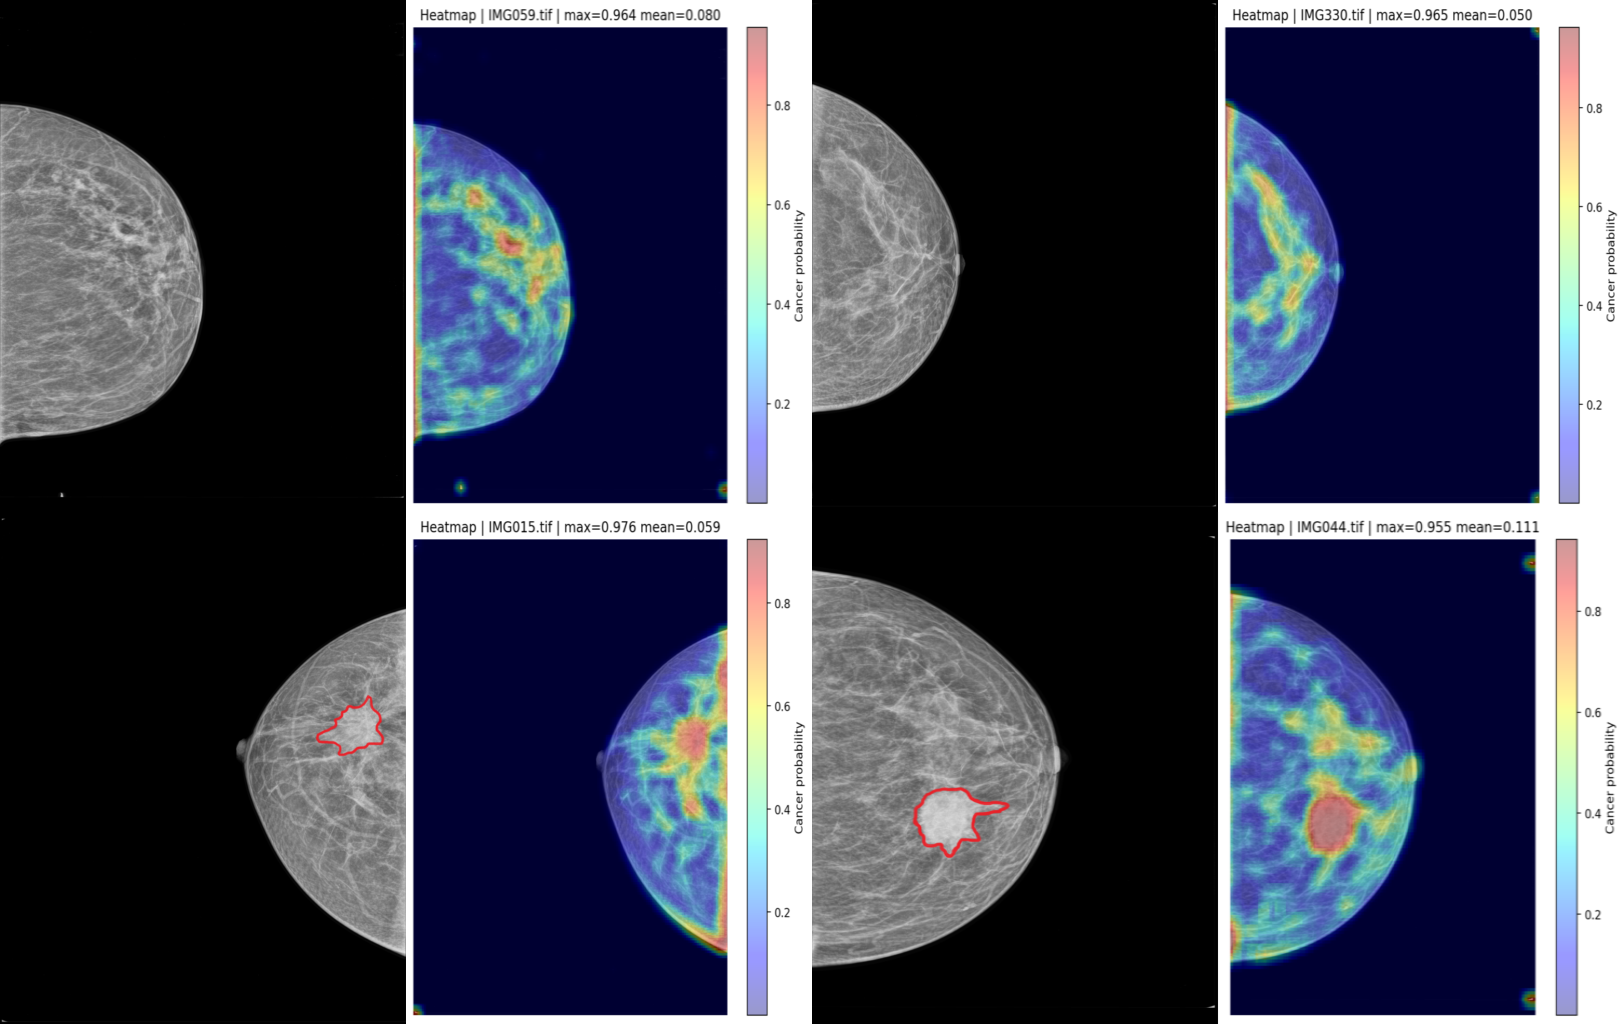
\includegraphics[width=0.48\linewidth]{../results/exp_022_mmr_n10_k3/heatmaps_side_by_side.png}
    \caption{Heatmap summaries for two reduced-bank sparse variants. Even very small kernel banks can remain qualitatively informative, though their AUC trails the strongest larger-bank models.}
    \label{fig:reducedbankheatmaps}
\end{figure}

\section{Composition and QMC Sampling}
After sparse selection had been validated, the next step was to ask whether many useful kernels could be compressed into a smaller set of aggregate filters. Composition improves compactness and visual readability, but the compression happens before classification, so part of the discriminative signal is lost. In the strongest composition setting used here, the composite model reaches test AUC 0.8933 and test accuracy 0.8150.

What remains consistent across the composition studies is the qualitative conclusion: composition can produce compact and visually meaningful filters, but it often falls short of the non-compressed selected-kernel classifier because nonlinear response pooling makes pre-classification compression lossy.

Figure~\ref{fig:compositegrid} shows a representative composite-kernel panel from this stage. These filters are easier to inspect than hundreds of separate kernels, but the numerical gap confirms that compactness alone is not enough; how the composition is constructed matters.

\begin{figure}[H]
    \centering
    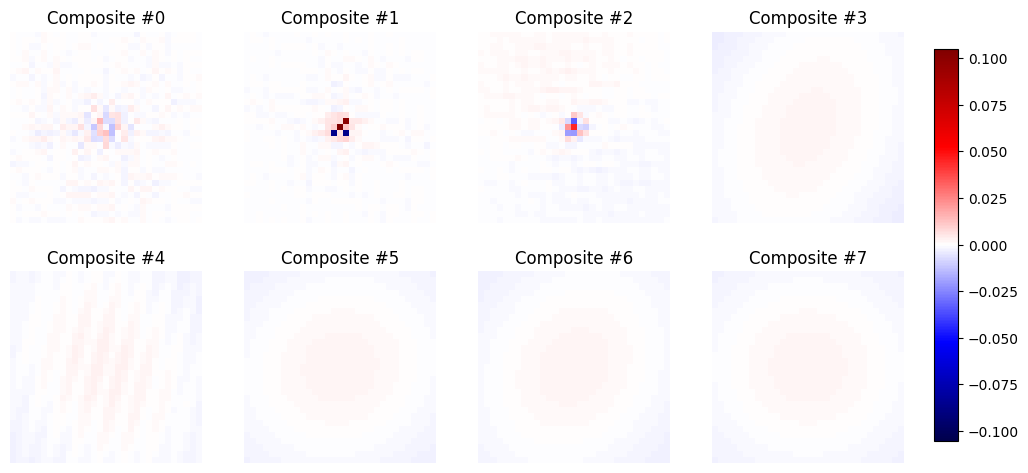
\includegraphics[width=0.92\linewidth]{../results/exp_022/composite_kernels_grid.png}
    \caption{Composite kernel grid from the rotation/composition experiments. Composition improves compactness and visual interpretability, but usually compresses away some discriminative information.}
    \label{fig:compositegrid}
\end{figure}

The next improvement targeted search rather than compression. Replacing random parameter draws with Sobol quasi-Monte Carlo sampling gives the cleanest matched gain in the thesis because it changes only how the kernel space is explored. Table~\ref{tab:qmc} summarizes the key comparison.

\begin{table}[H]
\centering
\caption{Matched random-versus-QMC comparison.}
\label{tab:qmc}
\begin{tabular}{lccc}
\toprule
Evaluation & Random sampling & QMC sampling & QMC - Random \\
\midrule
Base model AUC & 0.9195 & \textbf{0.9387} & +0.0192 \\
Composite model AUC & 0.8855 & \textbf{0.8934} & +0.0080 \\
Composite model ACC & 0.8063 & \textbf{0.8176} & +0.0114 \\
\bottomrule
\end{tabular}
\end{table}

This is one of the strongest results in the thesis because it isolates a single design choice. No new classifier is introduced and no heavier model is used. The improvement comes from covering the kernel-parameter space more effectively. For a low-volume regime, this is precisely the kind of gain that adaptive design aims to achieve.

\section{Rotation Sensitivity and Enforced Invariance}
The next step examined whether orientation should be modeled explicitly. The first observation was that the learned composite filters were not intrinsically rotation invariant, yet the change under right-angle rotations was relatively small. This suggested that response pooling already provides some practical robustness.

To test strict invariance, the kernel was then averaged over rotated copies. This yields exact right-angle stability by construction. On one evaluation split, the invariant kernel reaches test AUC 0.8908 and test accuracy 0.8091, with identical values at $0^\circ$, $90^\circ$, $180^\circ$, and $270^\circ$. On a regenerated patch split, the same behavior remains, with test AUC 0.8755 and test accuracy 0.8006.

Figure~\ref{fig:rotation} summarizes the angle-by-angle behavior. The key lesson is not simply that invariance is possible. It is that enforcing invariance trades some discriminative freedom for predictable behavior.

\begin{figure}[H]
    \centering
    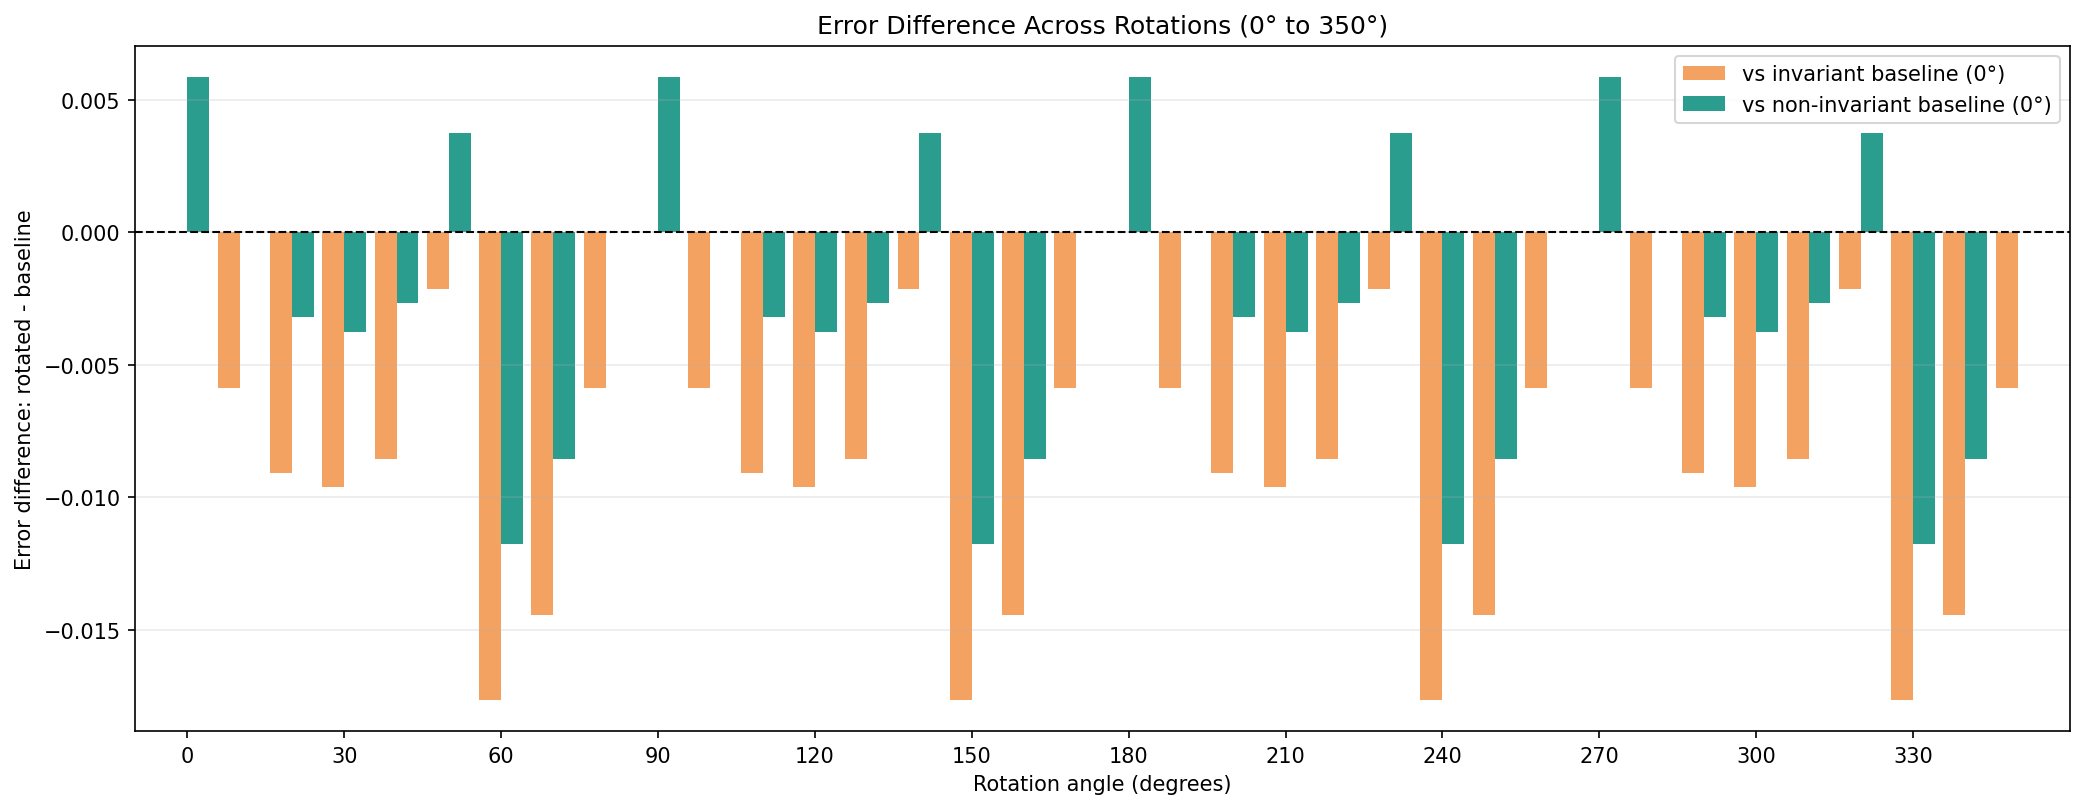
\includegraphics[width=0.9\linewidth]{../Reports/figures/rotation_error_difference_barplot.png}
    \caption{Rotation robustness of an explicitly averaged invariant kernel over angle sweeps. The comparison shows that invariance can be enforced exactly, but with some cost in discriminative performance.}
    \label{fig:rotation}
\end{figure}

\section{Chronological Development of the Radial Models}
The radial line of work is the most important part of the thesis because it turns a large heterogeneous bank into a compact structured model. The development is best understood as a sequence of problems and fixes.

The first radial model was obtained by circularizing a previously learned kernel and reading out one coefficient per radius shell. This seed kernel already performed reasonably well, with test AUC 0.8825 and test accuracy 0.8000, which showed that a one-dimensional radial profile could still capture meaningful lesion structure.

The next step optimized the shell coefficients directly from that seed. This improved the radial model to test AUC 0.9151 and test accuracy 0.8449, but it also exposed a problem: the learned profile developed a narrow spike and remained strongly influenced by the initialization. The issue was not only numerical. It made the kernel harder to interpret because the optimizer could rely on a sharp shell preference inherited from the seed.

To reduce that ambiguity, a signed compact version was introduced. This model switched to a signed response and controlled the support more directly. The result was more stable but also more conservative, with test AUC 0.8885 and test accuracy 0.8118.

The next improvement removed dependence on the old seed entirely. An independent signed radial model was learned from scratch with a signed top-$k$ response and explicit normalization. This solved the initialization problem, but a new issue became visible: when positivity and monotonicity were enforced too strongly, the kernel behaved too much like an averaging filter over bright tissue. That made the representation cleaner, but also too restrictive.

To test whether that restriction was the real bottleneck, positivity and monotonicity were removed in a free signed radial ablation. This restored positive and negative structure, but the unconstrained profile became less stable and dropped to test AUC 0.8864 and test accuracy 0.8096. The lesson was that signed freedom was necessary, but some structural control was still needed.

The final model resolves this trade-off by learning both the signed shell values and the effective kernel size. The shell coefficients remain normalized, but they are allowed to be positive or negative, and a differentiable radius parameter changes the effective support through radial rescaling and a soft support gate. The classifier still uses the signed top-$k$ response, while smoothness, curvature, and outer-shell penalties prevent unstable profiles. The learned effective radius is about 13.18 shells, and the final model reaches test AUC 0.9101 with test accuracy 0.8449.

This final stage is the thesis endpoint because it is the most complete formulation of the original goal: a compact radial kernel whose values are interpretable, whose size is learned rather than fixed by hand, whose score depends on signed structure rather than absolute brightness, and whose normalization keeps the representation comparable across optimization steps.

The geometric ablations help justify the radial prior. When the radial structure is replaced by more generic geometric templates, performance falls clearly: the non-circular geometric model reaches test AUC 0.8109 and test accuracy 0.7358, while the square-only version reaches test AUC 0.7995 and test accuracy 0.7353. This shows that the circular prior is not arbitrary. It matches the morphology of the case study better than the harder-edged geometric alternatives.

\begin{figure}[H]
    \centering
    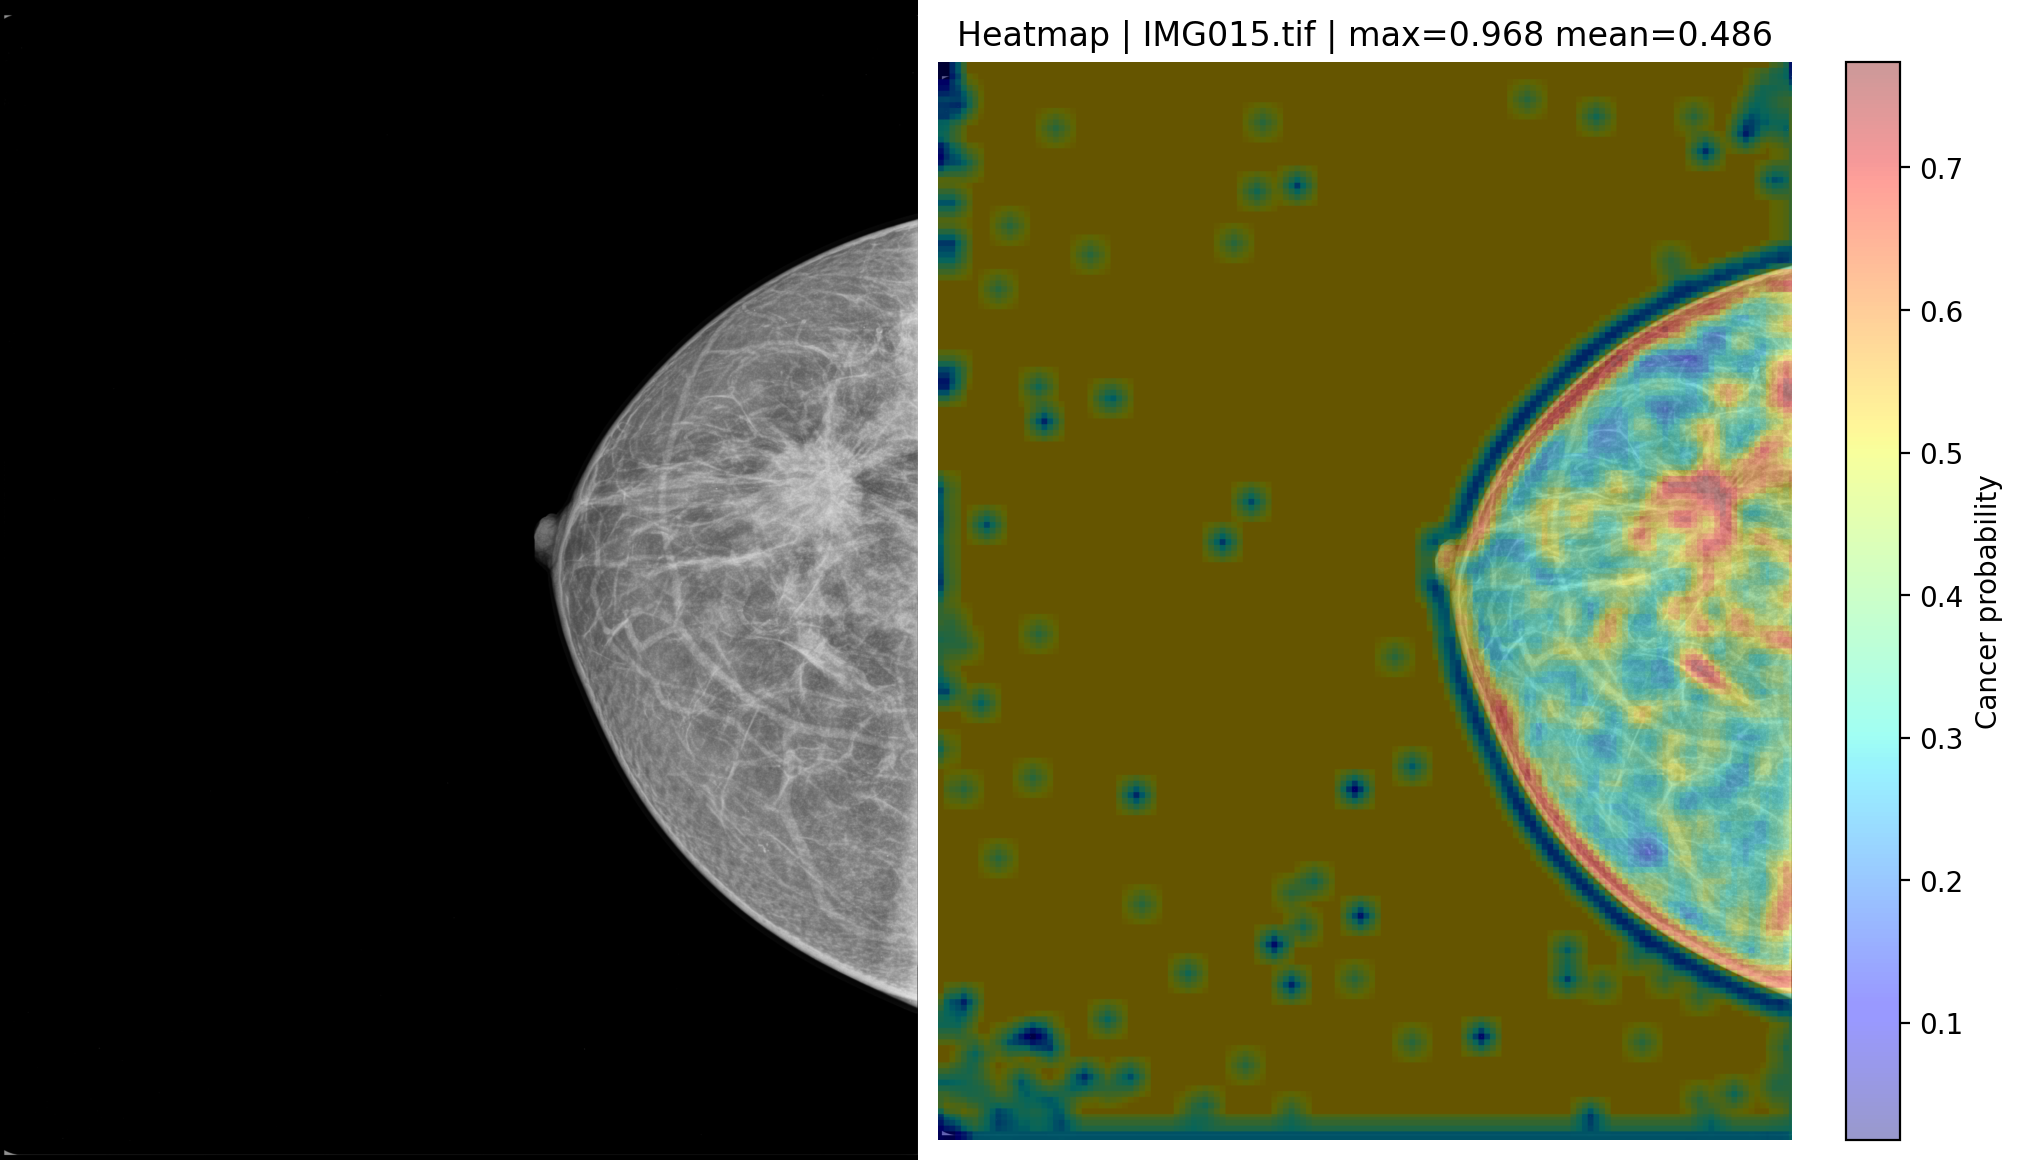
\includegraphics[width=0.48\linewidth]{../results/triangular_square_shape_sensitive/exp_001/heatmaps_pairs/IMG015_pair.png}\hfill
    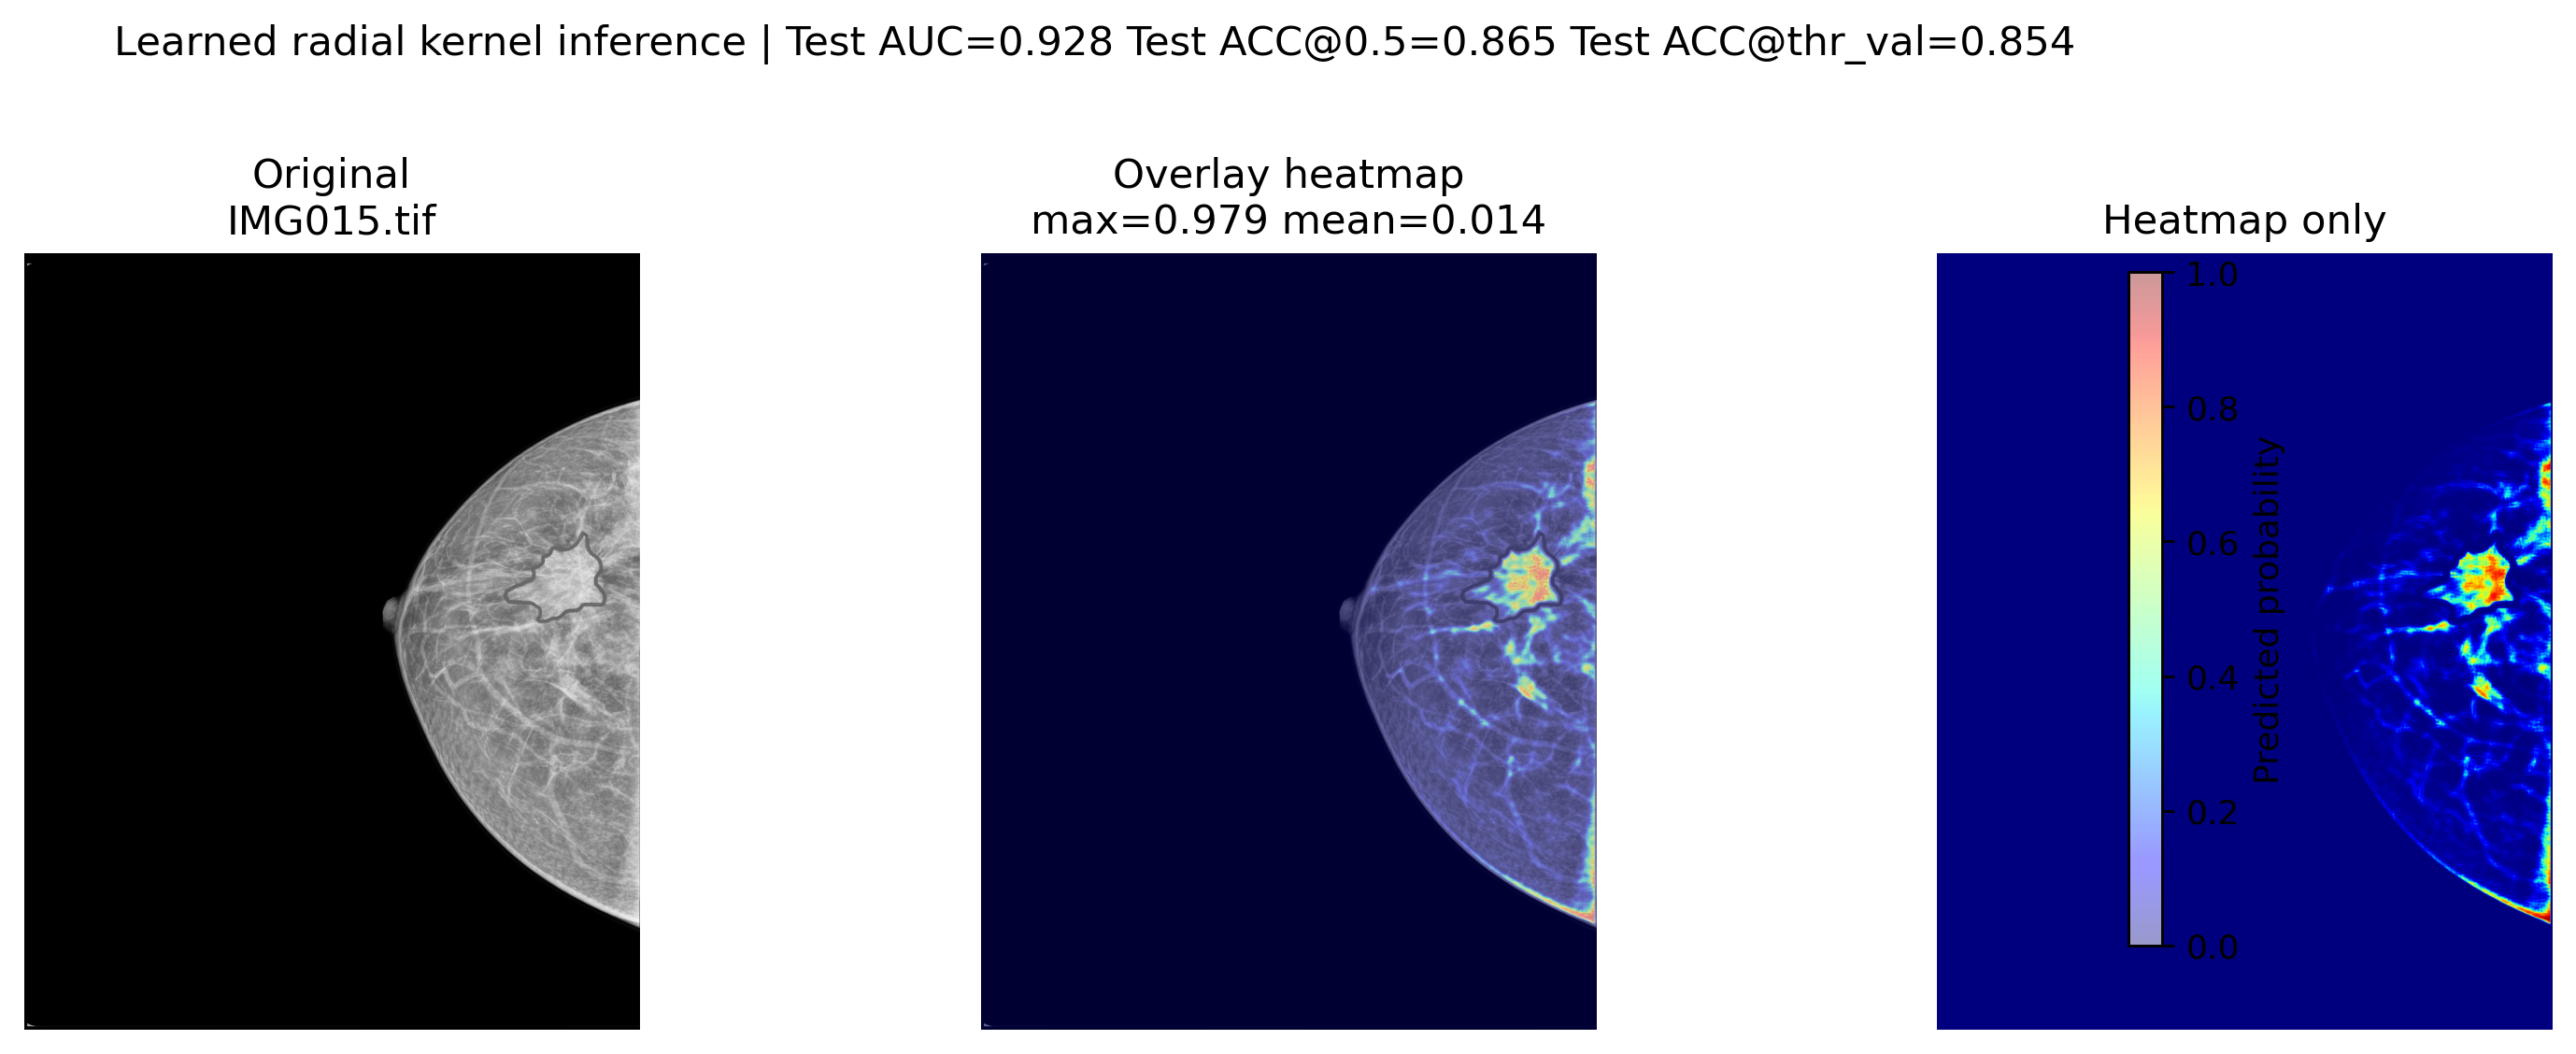
\includegraphics[width=0.48\linewidth]{../Reports/figures/radial_single_kernel_heatmap.png}
    \caption{Geometric ablation versus radial heatmap comparison. The geometric model spreads probability broadly across boundaries and texture, whereas the radial model is more selective around the suspicious region.}
    \label{fig:triangularradialcompare}
\end{figure}

\section{Interpreting the Radial Transition}
Two observations explain why the radial development required several redesigns. First, the spike in the early seed-based fit was not evidence of a uniquely meaningful lesion ring. It came from the optimization setup: a non-neutral seed, weak smoothness control, and a pooled score that over-rewarded isolated large activations. This is exactly why later signed and scratch-trained models were introduced.

Second, visually different kernels can still produce similar classification behavior when the response map is compressed to one or a few scalar values. The later signed top-$k$ formulation was introduced partly to reduce that ambiguity and make the score depend on a more consistent signed pattern rather than on one dominant absolute peak.

Figure~\ref{fig:radialsummary} shows the final learnable-radius radial model, and Figure~\ref{fig:radialheatmap} shows a representative heatmap from the signed radial development line.

\begin{figure}[H]
    \centering
    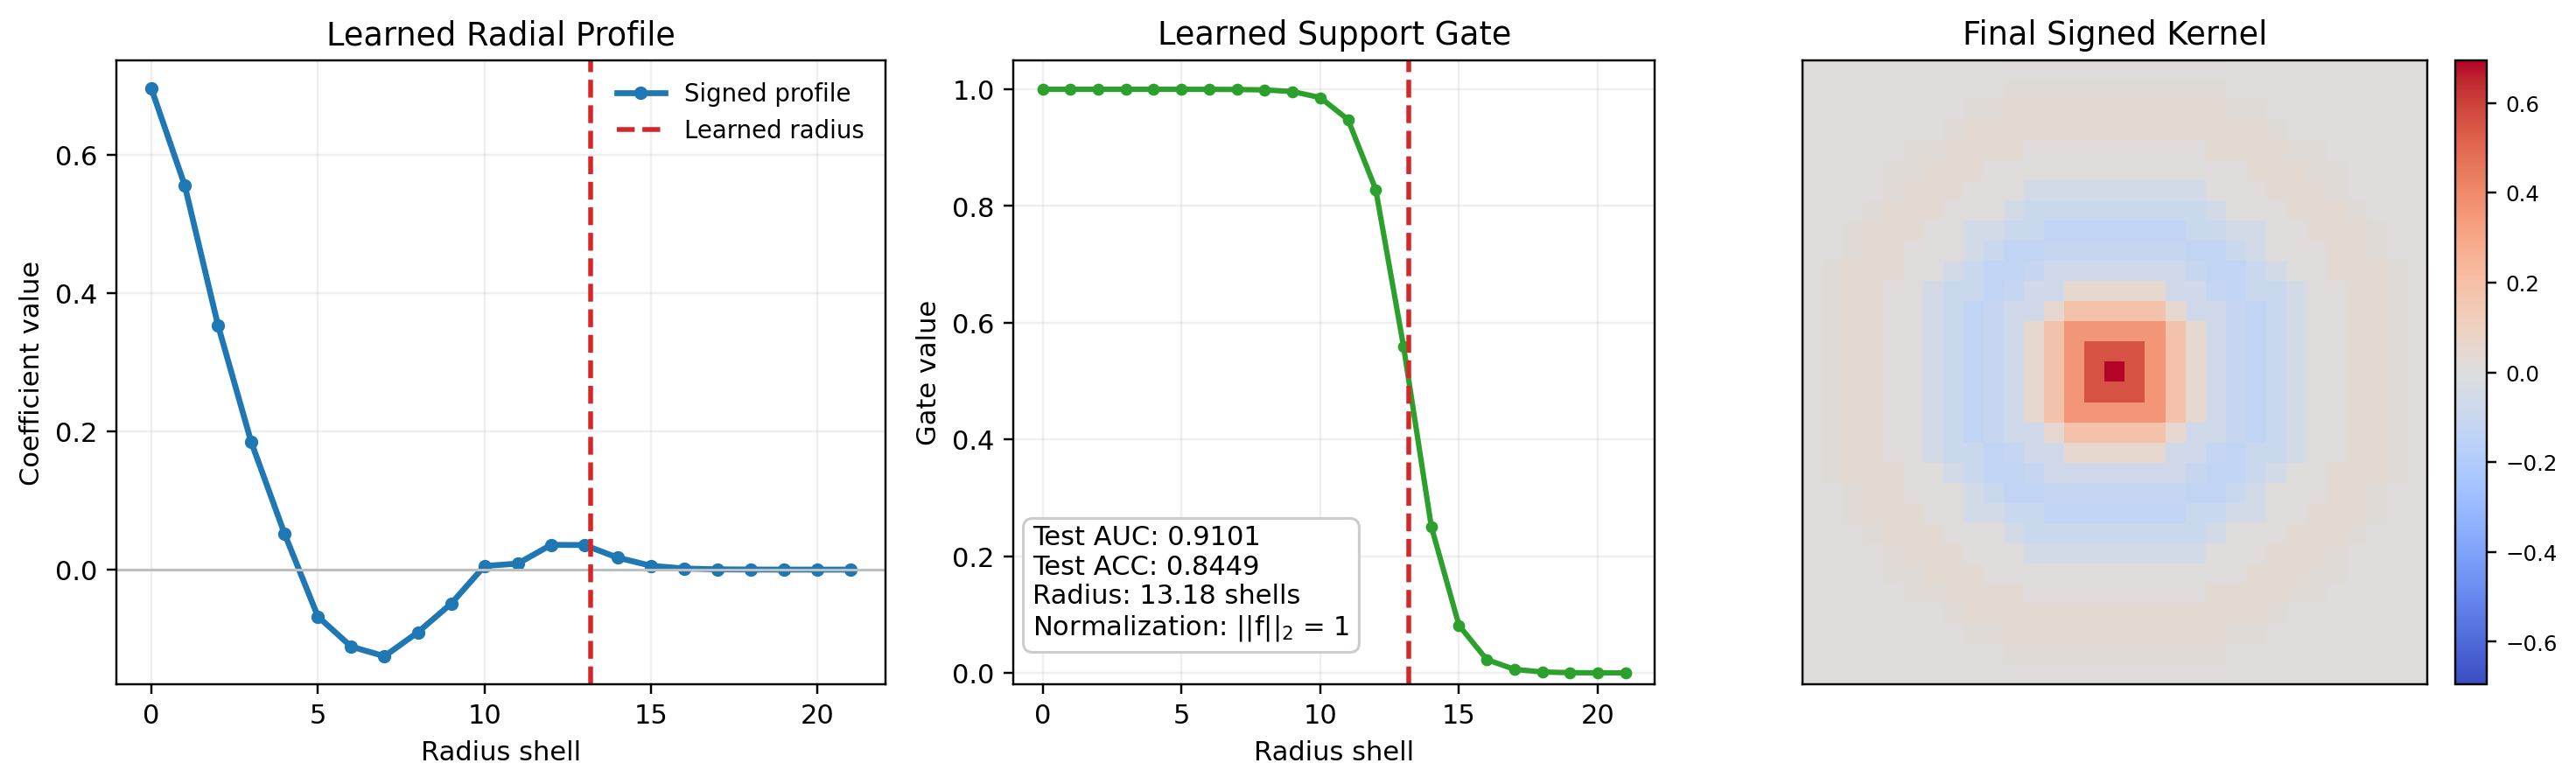
\includegraphics[width=0.96\linewidth]{../Reports/figures/radial_learnable_radius_summary.png}
    \caption{Final learnable-radius radial model. The summary shows the signed normalized profile, the learned support gate, and the resulting kernel.}
    \label{fig:radialsummary}
\end{figure}

\begin{figure}[H]
    \centering
    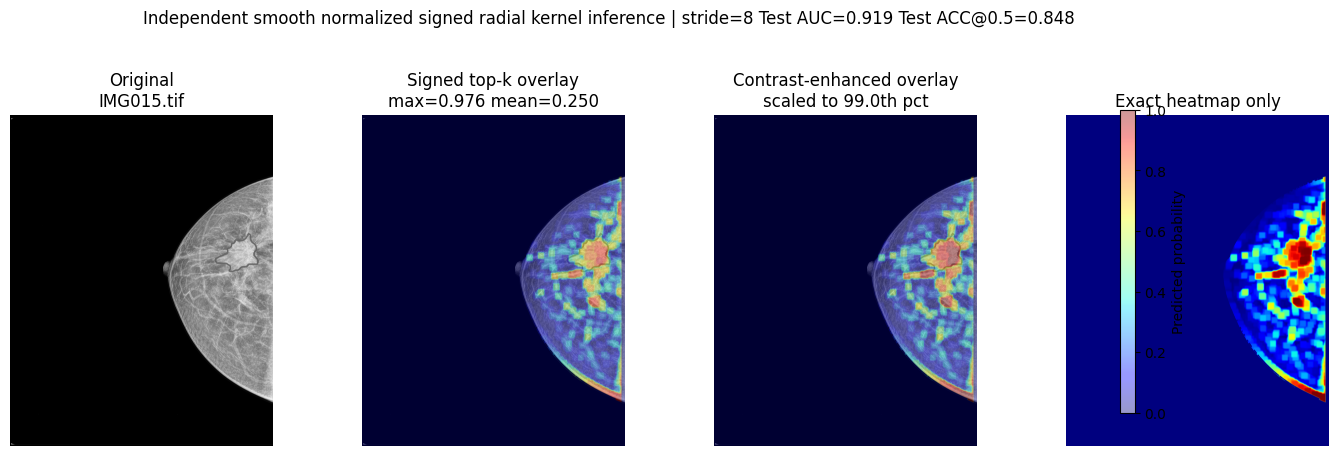
\includegraphics[width=0.96\linewidth]{../Reports/figures/radial_kernel_from_scratch_heatmap.png}
    \caption{Representative heatmap from the signed radial family. The qualitative output supports the claim that compact radial filters can remain spatially meaningful.}
    \label{fig:radialheatmap}
\end{figure}

\section{Synthesis}
The experiments support four main claims.

\subsection{Adaptive kernel design is viable for low-volume medical data}
Across bank selection, QMC search, composition, rotation-aware kernels, and radial fitting, the project repeatedly reaches strong patch-level AUC values while using small classifiers and explicit filters. The representation is therefore not merely a handcrafted baseline; it is a competitive learning strategy in its own right.

\subsection{Not every adaptation improves the same property}
The project does not support a simplistic ``more adaptation is always better'' conclusion. QMC sampling improves matched performance. MMR selection provides sparse, strong baselines. Composition improves compactness and visualization, but often reduces performance. Rotation averaging gives exact invariance, but loses some discriminative detail. The thesis therefore interprets adaptation as a toolbox of trade-offs rather than a single monotone ladder.

\subsection{Stronger priors help when they match the image structure}
The radial results and geometric ablations strongly suggest that circularly structured kernels match the lesion morphology of this case study better than generic geometric alternatives. This is an important result for low-data learning: a good prior can replace a significant amount of parameter freedom.

\subsection{The final learnable-radius radial model is the best thesis endpoint}
The final signed radial model with learnable effective radius is the most defensible \emph{thesis contribution} because it addresses identifiability, stability, support selection, and interpretability within one compact formulation. The project therefore ends not with the loosest radial score, but with the most structured signed formulation that still remains strongly competitive.

\chapter{Conclusion}
This thesis examined the problem of optimal classification under low-volume medical data conditions through the lens of adaptive kernel design. The case study was a local mammographic image dataset with pixel-level annotations and patch-level lesion/background sampling. Instead of relying on a single large model, the work adapted the representation at multiple levels: kernel-family selection, diversity-aware ranking, kernel composition, low-discrepancy parameter sampling, rotation-aware construction, and compact radial parameterization.

The results support a clear overall answer to the thesis question. Adaptive kernel design is a viable strategy for low-volume medical image classification when accuracy, interpretability, and controllable priors all matter. Better search over the kernel space improves the bank-based baseline, kernel composition improves compactness but usually sacrifices some discrimination, and explicit rotational averaging clarifies the robustness-versus-discrimination trade-off. The most important outcome is the radial line of work, which shows that one can move from a broad filter bank to a compact signed radial model that also learns its effective size. The final formulation reaches test AUC 0.9101 and test accuracy 0.8449 while remaining far more structured and interpretable than the original bank-based representation.

The thesis therefore contributes an \emph{adaptive kernel design framework} rather than a single isolated algorithm. The framework begins with explicit filter banks and progressively injects stronger prior structure until the representation itself becomes a one-dimensional radial profile. This makes the final model easier to interpret, easier to regularize, and better aligned with the low-data regime motivating the work.

The final learnable-radius radial result is shown in Figure~\ref{fig:finalradial}. It summarizes the signed normalized profile, the learned support gate, and the resulting kernel for the final model. This result matters for three reasons. First, it ties accuracy to a structured, signed radial shape rather than to an absolute-peak artifact. Second, the learned support radius removes hand-tuning of kernel size while preserving interpretability. Third, the unit-normalized parameterization makes the learned filter comparable across runs, which is essential for principled low-data analysis. The model reaches test AUC 0.9101 with test accuracy 0.8449, which keeps performance competitive while significantly tightening the inductive bias.

\begin{figure}[H]
    \centering
    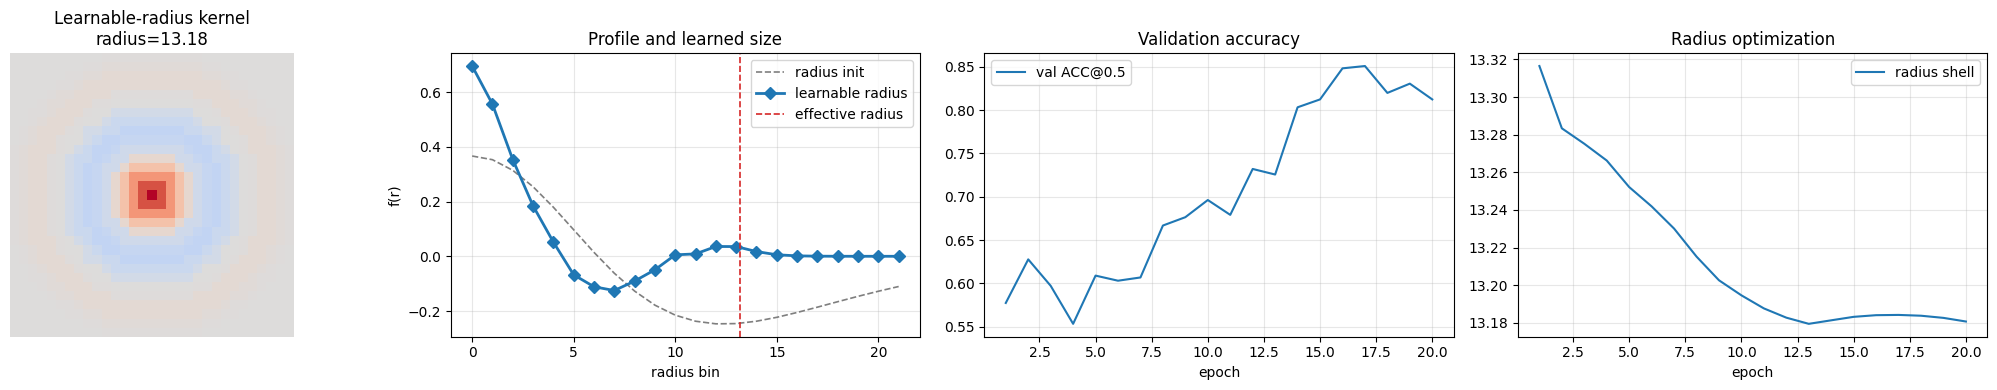
\includegraphics[width=0.96\linewidth]{../Reports/figures/radial_learnable_radius_multi_panel.png}
    \caption{Final learnable-radius radial result. The figure summarizes the learned kernel, radial profile with learned size, validation accuracy, and radius evolution.}
    \label{fig:finalradial}
\end{figure}

Several directions remain open. The most immediate next step is a unified rerun of the strongest bank, composition, QMC, and radial configurations on one fixed split so that all reported metrics become directly comparable. Additional future work should include cross-validation, patient-level evaluation beyond patch classification, deeper comparison with compact deep-learning baselines, and hybrid models that combine kernel priors with learned feature heads.

In summary, the thesis shows that low-volume medical image classification does not have to default to opaque high-capacity models. Carefully designed adaptive kernels can provide competitive performance, explicit visual semantics, and a principled path toward compact interpretable models.

\bibliographystyle{plainnat}
\bibliography{master_thesis}

\end{document}
